\chapter{Определение смысловой близости пары ключевых слов} \label{chapt_word_similarity}
% SYNOPSIS_2 >>>
В настоящей главе подробно описываются разработанные автором эвристические модели, алгоритмы и реализующее их программное обеспечение для определения семантической близости пары ключевых слов. Разработанные автором на основе проведенных исследований с использованием полученных в их ходе эвристических соображений модели определения семантической близости являются важным результатом деятельности в рамках подготовки настоящей диссертации.

Задача, решение которое представлено в данной главе, имеет следующую математическую постановку. Дано множество объектов системы $D$ и множество ключевых слов $W$, множество наборов ключевых слов $T$. Каждый элемент $d_i \in D, i=1\ldots N$ представлен \emph{набором ключевых слов} $t_i \in T$, состоящим из  $k_i$ ключевых слов из множества $W$:

$$d_i\rightarrow t_i = (w_{i_1},w_{i_2},...,w_{i_{k_i}}).$$

Множество $T$ состоит из \emph{уникальных наборов ключевых слов}. Наборы ключевых слов совпадают, если существует перестановка, отождествляющая эту пару наборов. Кроме того, между объектами системы заданы отношения различных типов, определенные направленным графом $G_{rel} = (D, R)$, в котором $D$ - множество вершин (объекты системы), а $R$ - ребра, определяющие отношения. Ребра этого графа помечены типом отношения: $l: R \rightarrow T$, где $T$ - множество возможных типов.  Множества $(D, T, W, G_{rel})$ задают модель информационной аналитической системы.

В рамках данной главы необходимо будет представлена модель определения семантической близости и в ее рамках такая функция близости $f : W \times W \rightarrow [0, 1]$, б\'ольшие значения которой означают сильный уровень смысловой близости между ключевыми словами.

Для определения семантической близости вводятся вспомогательные графы, вершинами которых являются ключевые слова, а ребра указывают на некоторые свойства пары ключевых слов. В самом простом виде таким свойством может являться факт причастности пары ключевых слов одному набору. Кроме этого существуют более сложные и неявные связи между парами ключевых слов. Примером такой связи может служить \emph{контекстная близость}, определенная в главе \ref{cont_sim}. Согласно введенной модели, такая близость устанавливается между парой ключевых слов $w_a$ и $w_b$ в том случае, если существует большое число ключевых слов, которые входят одновременно и в наборы, содержащие слово $w_a$, и в наборы, содержащие слово $w_b$. Этот факт означает, что если для пары слов существует достаточное количество общих <<соседей по набору>>, то между ними проявляется такая контекстная связь.
% <<< SYNOPSIS_2 

Следует отметить, что \emph{контекстная близость} по результатам тестовых испытаний, приведенных в разделе \ref{cont_sim_experiment}, оказалась весьма точным способом приближения близости семантической. Этот факт означает, что данная мера близости может заменять разработанную в настоящей главе семантическую близость в ряде практических задач, в которых по каким-либо причинам нет возможности применеть более сложные моделей. Такими причинами могут являться ограниченность объема исходных данных, необходимость в использовании вычислительно более простой модели, отсутствие какой-либо информации, кроме коллекции наборов ключевых слов и другие.

На основе разработанной в данной главе модели контекстной близости \emph{WordContSim}, автором был разработан алгоритм кластеризации множества ключевых слов информационной системы. Результаты по данному направлению описываются далее в разделе \ref{clustering}.

Еще одним способом получать связи между ключевыми словами является использование новых источников данных, поставляемых рассматриваемой информационно-аналитической системой. В рамках наукометрических систем такими источниками могут служить данные о конференциях, публикациях, проектах и других сущностях системы, если с ними ассоциируются ключевые слова. Связи такого рода не обязаны напрямую влиять на семантическую близость пары слов, для которой они проявляются. Например, пара ключевых слов, используемая одновременно двумя сотрудниками одного факультета в своих научных работах, не должна обладать семантической близостью. Тем не менее, такая информация при учете других факторов может нести дополнительный сигнал для модели определения семантической близости.

Большое количество различных характеристик, связей и источников данных различной природы затрудняет процесс определения близости. Эвристические подходы для выбора окончательных формул семантической близости являются менее эффективными и сложнореализуемыми. Причиной этому является необходимость вручную подбирать математическое выражения, учитывающие большое число различных аспектов близости. Для преодоления этой трудности автором настоящей диссертации предлагаются подходы, основанные на применении методов машинного обучения. Подробное их описание представлено в разделе \ref{ml_sim}. По результатам исследований и тестирования программных реализаций, такие подходы в значительной мере улучшают качество определения смысловой близости между ключевыми словами. 

С помощью известных алгоритмов теории графов, среди которых присутствуют поиски кратчайших путей, нахождения потока между вершинами, определения мер центральностей вершин и другие теоретико-графовые подходы, появляется возможность количественно охарактеризовать рассматриваемую пару вершин внутри построенных графов. Кроме этого, используется новая разработанная автором числовая характеристика меры абстрактности ключевого слова, описанная в \ref{abstractness}. Эти числовые характеристики служат описанием (так называемым признаковым описанием объектов). Полученная информация используется для более точного определения семантической близости пары слов.

В связи с использованием методов машинного обучения с учителем для лучшего определения уровня смысловой близости, возникает необходимость сбора обучающей информации для подлежащих обучению моделей. В настоящей работе описывается новый алгоритм автоматического формирования обучающей выборки для проведения обучения. Важность такого алгоритма, описанного в разделе \ref{art_train}, заключается в том, что он избавляют от необходимости ручной разметки данных, которая обычно является ресурсозатратной.

В заключительной части главы представлены результаты и выводы относительно разработанных автором моделей определения семантической близости для пары ключевых слов.

\section{Модель семантической близости \emph{WordContSim}} \label{wordcontsim}
% SYNOPSIS_2.1 >>>
В данном разделе описывается модель близости, названная \emph{WordContSim}. Начало раздела посвящается введению вспомогательного графа ключевых слов, после чего приводится описание и аргументация эвристических идей, заложенных в данную модель. Следующим этапом изложения является представление реализающих данную модель алгоритмов, асимптотических оценок вычислительной сложности и затрат по памяти для их программных реализаций.
% <<< SYNOPSIS_2.1

\subsection{Построение графа ключевых слов} \label{sect1_1}

В основе модели вычисления семантической близости \emph{WordContSim} лежит построение специального взвешенного \emph{графа ключевых слов} $G_{kw}(W, E_{mut})$, вершинами $W$ которого являются ключевые слова системы, а ребра $E_{mut}$ - отражают факт вхождения пары ключевых слов в один набор. Вершину, соответствующую ключевому слов $w$ обозначим за $v_w$. Вес ребра отражает в простейшем виде смысловую связь между соответствующими ключевыми словами и  задается формулой:
\begin{equation}\label{tag_graph_weight}
\omega(v_{w_i}, v_{w_j}) = \sum_{\{t \in T : w_i \in t , w_j \in t\}}\frac{1}{|t|},
\end{equation}
где $|\cdot|$ обозначает количество ключевых слов набора.

Выбор формулы, определяющей вес ребра, объясняется следующими двумя соображениями.
\begin{enumerate}
    \item Чем чаще пара слов встречается в одном наборе, тем более вероятна их семантическая связь и тем больший вес ставится соответствующему ребру.
    \item Чем больше слов содержит набор, тем менее вероятно, что два рассматриваемых слова семантически связаны непосредственно друг с другом, а не с другими словами набора. Поэтому набор, состоящий из большего числа слов, вносит меньший вклад в вес ребра.
\end{enumerate}

Кроме этого, помечаются вершины описанного графа. Каждой вершине приписывается количество упоминаний в коллекции ассоциированного с этой вершиной ключевого слова:

$$ \upsilon(v_w) = |\{t : w \in t, t \in T\}| $$

Характеристика совместной встречаемости внутри одного набора является важной для определения семантической близости, но не определяющей: слова одного набора не обязаны быть похожими друг на друга по смыслу. Напротив, нередко они служат для того, чтобы более точно описать общую тему документа, к которому относятся, а добавление точного синонима не добавляет информации о тематике документа. 

Использование формулы \ref{tag_graph_weight} в качестве меры семантической близости протестировано вместе с другими моделями вычислений. Результаты тестирования программной реализации модели, основанной на данной формуле, представлены в \ref{cont_sim_experiment}. Качество такой модели заметно уступает более сложным моделям, существенно использующим семантику. Несмотря на этот факт, введенный выше \emph{граф ключевых слов} является необходимой структурой данных для определения контекстной меры близости, описание которой следует разделе \ref{cont_sim}. Здесь и далее граф ключевых слов будет обозначен через $G_{kw}$

\subsection{Контекстная модель определения семантической близости для пары ключевых слов} \label{cont_sim}

Для введения понятия \emph{контекстной близости} рассмотрим подграфы введенного ранее графа ключевых слов, изображенных далее.

\begin{figure}[ht]
  \begin{minipage}[ht]{1.0\linewidth}\centering
    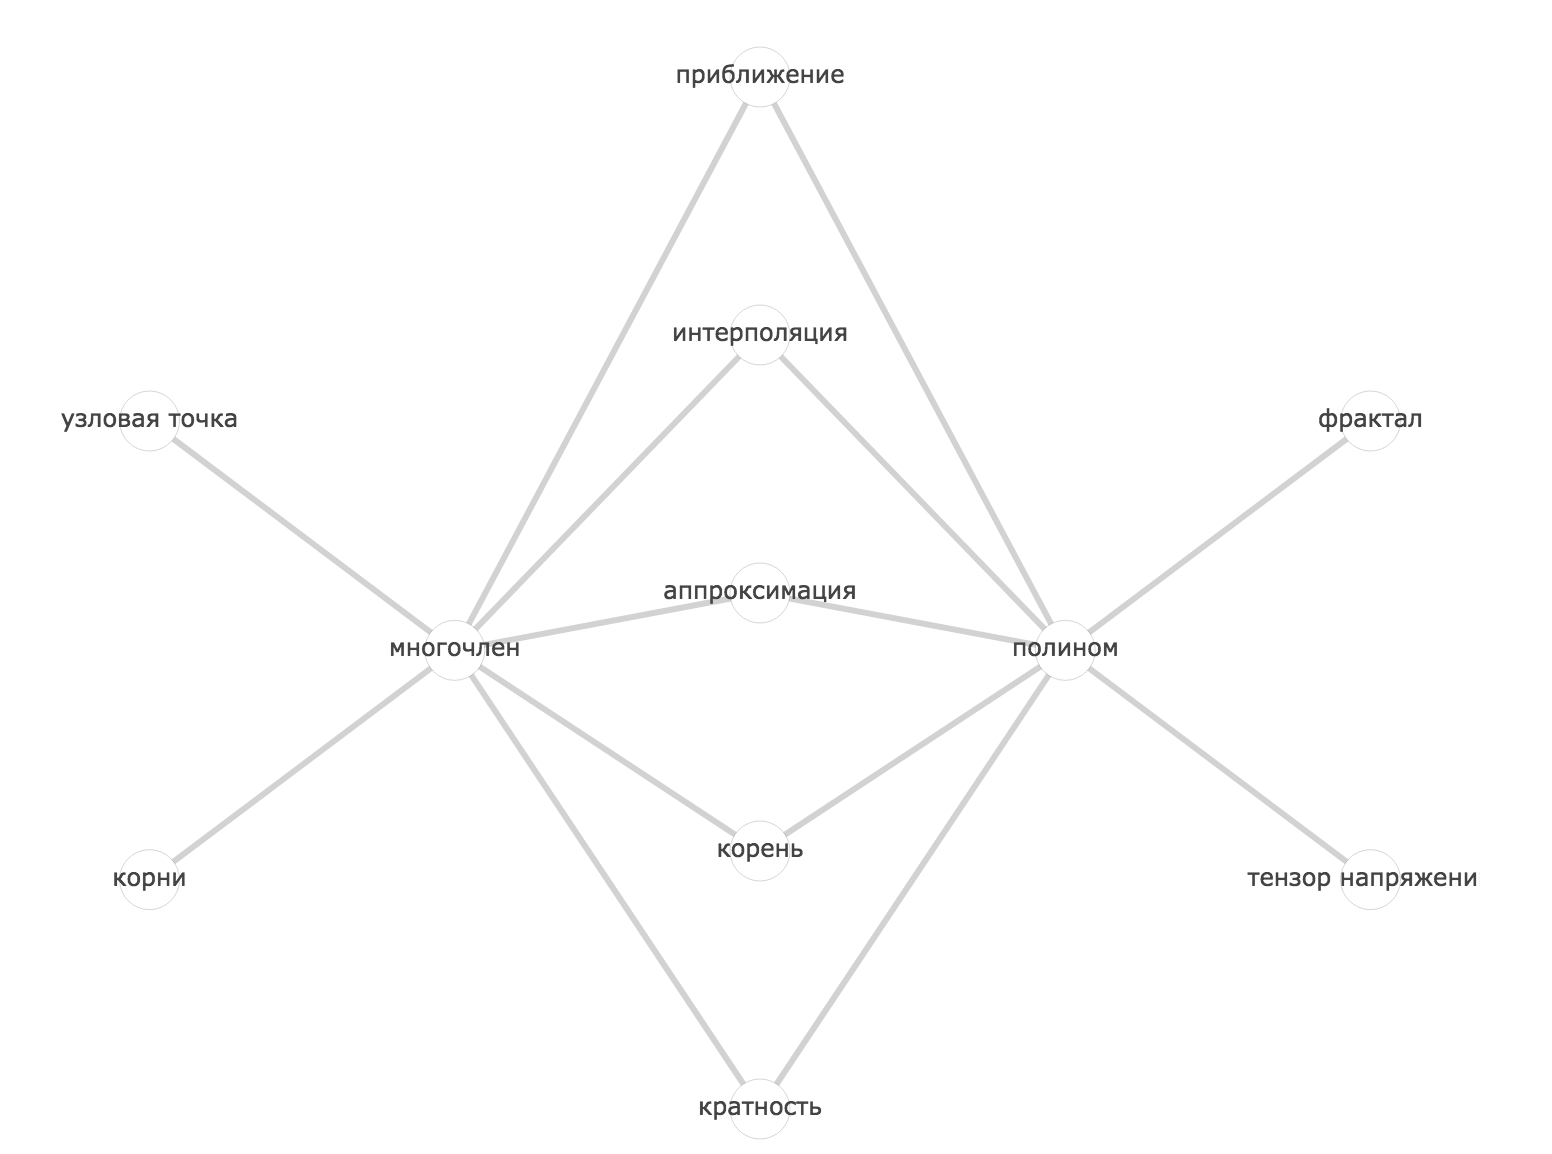
\includegraphics[width=1.0\linewidth]{Dissertation/pics/polynom}
    \caption{Соседи вершин <<полином>> и <<многочлен>> в графе ключевых слов}
    \label{img:abstr_hist}
  \end{minipage}
\end{figure}

Проанализиров изображение, можно отметить следующий факт: пара вершин, ассоциированных со словами <<многочлен>> и <<полином>> не входят ни в один набор ключевых слов коллекции (поскольку в графе отсутствует ребро между этими вершинами), но имеет при этом большое число общих соседей. Поскольку эти два слова действительно семантически близки (являются синонимами), то это наводит на идею использования такой характеристики для пары вершин в качестве одной из компонент в формуле, позволяющей вычислять меру семантической близости.

Другими словами, отмечается следующее наблюдение: уровень семантической близости слов $w_x$ и $w_y$ тем больше, чем больше у вершин $v_{w_x}$, $v_{w_y}$ общих соседей в \emph{графе ключевых слов}. Соответствующее множество слов $\mathcal{C}_{T;w_x, w_y}$ для этих вершин записывается в следующем виде: $\mathcal{C}_{T;w_x, w_y} = \{w | (w, w_x) \subset t_i, (w, w_y) \subset t_j, (t_i, t_j) \in T, i \neq j\}$ и обозначается \emph{контекстным множеством для ключевых слов $w_x$ и $w_y$}. Название <<контекстное>> выбрано по той причине, что такое множество определяет в каком общем контексте употребляются  два ключевых слова в рамках одной коллекции. Чем больше мощность этого множества, тем более вероятна семантическая связь между словами $w_x$ и $w_y$.

После того, как контекстное множество определено, необходимо уметь получать по этому множеству численную характеристику близости. Для этих целей в рамках принятых ранее обозначений определена следующая формула:

\begin{equation}\label{context_raw}
    \hat{C}_T(w_i, w_j) = \sum_{w_i \in \mathcal{C}_{T;w_x, w_y}} \min(\omega(v_{w_x}, v_{w_i}), \omega(v_{w_i}, v_{w_y})).
\end{equation}

Согласно этой формуле, больший вклад в итоговый уровень близости дают те вершины графа ключевых слов, которые сильнее связаны с оцениваемой парой ключевых слов с точки зрения веса соответствующих ребер.

Следующим шагом в построении контекстной семантической модели близости является нормировка величины $\hat{C}_T(w_i, w_j)$. Дело в том, что формула \ref{context_raw} никак не учитывает частотности встречаемости оцениваемых слов в коллекции. Это обстоятельство приводит к тому, что значение, вычисленное по этой формуле, может оказаться большим, если рассматриваемые слова являются достаточно часто встречающимися (далее для краткости изложение - частотными) в рамках коллекции. Причина этому в том, что частотные слова имеют больше различных контекстов употребления и эти контексты с большей вероятностью будут сильнее пересекаться. При этом очевидно, что на семантическую близость такое свойство формулы влиять не должно. Поэтому уровень семантической близости должен быть обратно зависим от частотностей встречаемости рассматриваемых ключевых слов.


%Кроме того, поскольку слова $x$, $y$ и $k$ могут все входить в один набор, то в таком случае связь слов $x$ и $y$ через слово $k$ будет отражать скорее факт совместной встречаемости $x$ и $y$ в одном наборе, а не контекстную близость этой пары слов. Cовместная встречаемость далеко не всегда влечет сильный уровень семантической близости. Характер этой связи частотности и смысловой схожести во многом зависит от сферы, в которой применяются ключевые слова, и от того, с какой целью пользователи системы эти ключевые используют. Например, ключевые слова для научной публикации редко содержат в себе синонимы, поскольку эти слова используются для того, чтобы дать читателю понять о чем будет статья. Точные синонимы для слов в этом случае не несут никакой дополнительной информации о данной области. Вследствие этого, высокая частота совместной встречаемости не ведет к семантической близости и должна пессимизировать значение формулы контекстной близости. Другим примером являются ключевые слова в социальных сетях. Пользователи используют ключевые слова к документам таким образом, чтобы этот документ было легче найти среди других документов системы. Поэтому, использование синонимов, переводов, транслитерации, различных способов написания ключевых слов помогает в поиске документа. При этом, однако, не добавляет никакой смысловой информации непосредственно к описанию этого документа. Примеры различных наборов ключевых слов из разных областей будут даны в разделе <<Тестовые испытания>>. Исходя из этих соображений, предлагается две представленные далее формулы для вычисления контекстной близости для пары ключевых слов.

Для пары ключевых слов $w_i$, $w_j$ \emph{контекстная близость} определяется по формулам:

\begin{equation}
    \begin{aligned}
        C_T(w_i, w_j) = \frac{\hat{C}_{T}(w_i, w_j)}{f_{T}(w_i) + f_{T}(w_j)},\\
       %C_{\-}(i, j) = \frac{C(i, j)}{(1 + m(i,j)) * f(i) + f(j)},
    \end{aligned}
\label{eq:test}
\end{equation}
где $f_{T}(w_i)$- частота встречаемости слова $w_i$ в коллекции $T$.

Формула контекстной близости, введенная выше, показывает высокий уровень качества определения семантически близких пар ключевых слов. Кроме того, для оптимизации вычислений по формуле контекстной близости разработан алгоритм, эффективно вычисляющий значения для всех пар рассматриваемой коллекции. Описание этого алгоритма представлно далее. Вычислительная эффективность и высокий уровень качества получаемых результатов подтверждаются тестовыми испытаниями программной реализации модели, которые описаны в \ref{cont_sim_experiment}.

\subsection{Алгоритм вычисления значения контекстной близости по коллекции ключевых слов}

Кроме того обстоятельства, что вычисление контекстной близости имеет самостоятельный интерес, эта мера близости используется также для решения ряда других задач, рассматриваемы в рамках настоящей диссертации. Во-первых, формула контекстной близости необходима при расчете более сложной модели семантической близости, использующей методы машинного обучения (раздел \ref{ml_sim}). Во-вторых, она используется для решения задачи кластеризации ключевых слов (раздел \ref{clustering}).

В этой связи важным является умение эффективно предрассчитать (рассчитать в упреждающем режиме) значения меры близости для большого числа пар (например, для всех пар ключевых слов коллекции). Для этих целей автором разработан алгоритм, вычисляющий значения по формуле контекстной близости для пар рассматриваемой коллекции ключевых слов. Автором доказываются оценки на вычислительную сложность этого алгоритма и необходимые ресурсозатраты для его программной реализации.

Первым необходимым шагом для вычисления всех значений контекстной близости по коллекции $T$ является построение \emph{графа ключевых слов} $G_{kw}$, введенного ранее. \hl{Пусть граф ключевых слов хранится в виде массива хеш-таблиц. Индексы массива соответствуют номерам вершин, а хеш-таблица содержит отображение соседей задаваемой индексом вершины в значение веса соответствующего ребра}. Тогда следующее утверждение дает оценку вычислительной сложности построения графа ключевых слов.

\textbf{Утверждение 1.} Построение графа ключевых слов $G_{kw}$ по коллекции ключевых слов $T$ амортизационно  требует $O(|T|p^2)$ элементарных операций, где $p$ - максимальное число ключевых слов в одном наборе коллекции, $|T|$ - количество наборов в коллекции $T$.

Под амортизационным анализом здесь и далее понимается анализ средней производительности в худшем случае при усреднении по всем проводимым операциям.

\textbf{Доказательство.} 
\hl{В вершинах графа будем хранить не ключевые слова, а их уникальные числовые идентификаторы. Хранение графа организовано с помощью отображения идентификатора ключевого слова $x_{id}$ в другое отображение. Это внутреннее отображение, в свою очередь, ставит идентификаторам вершин соседей вершины $x_{id}$ в соответствии веса образованных ребер. Для этих целей наиболее подходящим является использование словаря, ключи которого являются целыми числами, а значениями - другой словарь. Ключами второго словаря также являются целые числа, а значениями - действительные числа. Внутренней структурой в реализации словаря и множества является хеш-таблица, что позволяет добиться амортизационно константного времени работы ($O(1)$) основных операций с этими структурами данных. Обозначим словарь верхнего уровня за $g$. Для хранения отображения ключевого слова в его уникальный идентификатор используется дополнительный словарь (хеш-таблица). Обозначим его за $w$.}

\hl{Кроме этого необходим дополнительный массив-счетчик $c$ для хранения количества упоминаний каждого ключевого слова в коллекции (по определению, в вершинах графа ключевых слов хранится эта характеристика). В ячейке с индексом $i$ в таком массиве будем хранить количество упоминаний в коллекции $T$ ключевого слова с идентификатором $i$. Идентификаторами служат целые числа от 0 до $n - 1$, где $n$ - число уникальных ключевых слов коллекции}.

\hl{Для заполнения структур $w$ и $c$ необходимо один раз рассмотреть каждое слово каждого набора коллекции. Если текущее слово уже имеет идентификатор (то есть существует запись в $w$), то нужно инкрементировать соответствующий счетчик в массиве-счетчике $c$. В ином случае нужно сначала добавить слово в словарь $w$, присвоив ему новый уникальный номер (номера считаются от нуля и каждый раз увеличиваются на единицу), а после этого добавить в массив $c$ новое значение, равное единице (что соответствует первому появлению слова в коллекции).}

\hl{Добавление в динамический массив и в хеш-таблицу, а также поиск в хеш-таблице  имеют амортизационную сложность $O(1)$. Доступ к элементу массива и инкрементация его значения имеют сложность $O(1)$. Эти операции проводятся для каждого слова каждого набора, которая в худшем случае оценивается, как $|T|p$ слов. Поэтому построение этих структур амортизационно имеет сложность $O(|T|p)$}.

\hl{Для построения графа необходимо рассмотреть все наборы коллекции и в каждом наборе рассмотреть все комбинации ключевых слов. Для каждой такой пары ключевых слов ($x$, $y$) необходимо найти их идентификаторы ($x_{id}, y_{id})$, а затем найти в словаре $w$ текущее значение веса ребра $w[x_{id}][y_{id}]$. Это значение необходимо инкрементировать на величину $\frac{1}{n_t}$, где $n_t$ - число ключевых слов в данном наборе. Если изначально такое значение в $w$ отсутствовало, то считать его равным нулю. Сложность всех этих операций амортизационно равна $O(1)$. Количество пар ключевых слов в худшем случае достигает $\frac{|T|(p-1)p}{2}$, если в каждом наборе оказалось ровно $p$ ключевых слов. Таким образом, сложность построения самой структуры графа амортизационно достигает $O(|T|p^2)$}.

\hl{Итак, общая вычислительная сложность амортизационно равна $O(|T|p^2 + |T|p) = O(|T|p^2)$}. Утверждение доказано.

Наивный подход, который рассчитывает меру близости для всех вершин графа ключевых слов заключается в переборе всех пар ключевых слов и вычислении общих соседей для каждой такой пары. По построенному пересечению и информации о частотностях слов вычисляется мера контекстной близости. Под частотностями, как и ранее, следует понимать количество упоминаний слова в коллекции $T$. Более подробно наивный алгоритм представлен далее.
\begin{enumerate}
    \item Построение графа ключевых слов $G_{kw}$.
    \item Инициализация разреженной матрицы $C$ размером $n * n$.
    \item Цикл по всем парам вершин $(v_{w_i}, v_{w_j})$ графа $G_{kw}$:
        \begin{enumerate}
            \item определение множества соседей для вершины $v_{w_i}$,
            \item определение множества соседей для вершины $v_{w_j}$,
            \item определение пересечения множеств соседей $\mathcal{C}_{T;w_x, w_y}$,
            \item вычисление $\hat{C}_T(w_i, w_j)$ по формуле \ref{context_raw},
            \item вычисление $C_T(w_i, w_j)$,
            \item сохранение значения в cоответствующей ячейке разреженной матрицы $C$.
        \end{enumerate}
    \item Матрица $C$ - возвращаемое алгоритмом значение.
\end{enumerate}

%%\hl{Назовем информационно-аналитическую систему \textbf{нетривиальной}, если количество уникальных 
Следующее утверждение доказывает оценку вычислительной сложности наивного алгоритма вычисления контекстной близости для пар ключевых слов коллекции.

\textbf{Утверждение 2.} \hl{При построенном графе ключевых слов} расчет весов всех пар ключевых слов наивным алгоритмом $C_T(w_i, w_j)$ имеет амортизированную сложность $O(n^2m)$, где $n$ - число вершин графа ключевых слов, $m$ - максимальное число ребер у вершины в графе ключевых слов.

\textbf{Доказательство.} 

Рассмотрим пару вершин графа. \hl{Поскольку сложность операции доступа к элементу хеш-таблицы в худшем случае равно $O(1)$, то сложность получения списков соседей в графе для каждой из этих вершин также амортизированно равна $O(1)$. Пересечение двух множеств занимает амортизированно $O(l)$, где $l$ - число элементов в меньшем из двух списков. В худшем случае сложность операции взятия пересечения амортизированно равна $O(m)$, если каждая вершина имеет $m$ соседей. Вычисление значений формул $C_T(w_i, w_j)$ также занимает $O(m)$. Поскольку число пар вершин квадратично по числу вершин и для каждой пары необходимо произвести $O(m)$ операций, то вычислительные затраты на подсчет значений оказываются равными $O(n^2m)$ Этот факт завершает доказательство}.

%Кроме этого перед началом вычислений необходимо построить граф ключевых слов. По утверждению 1 \hl{сложность этого построения равна} $O(|T|p^2)$. Следовательно, общее время работы алгоритма - $O(n^2m + |T|p^2)$. \hl{Этот факт завершает доказательство.}

%% неправда, что n > |T| !
%Далее, $m \ge p - 1$, так как набор из $p$ слов порождает клику из $p$ вершин с $p-1$ соседом в графе ключевых слов. Поэтому в худшем случае у вершины будет как минимум $p-1$ сосед. Из других наборов могли появиться новые соседи для данной вершины, поэтому $m \ge p $. В то же время $n \ge |T|$, поскольку наборы в коллекции уникальны и каждый набор состоит хотя бы из одного слова. Очевидно также, что $n \ge p$. Рассматривая произведение последних трех неравенств, получаем, что $n^2m > |T|p^2$, а значит, $O(n^2m + |T|p^2) = O(n^2m)$. Этот факт завершает доказательство.

%% n*m > |T| * p
%% 1 2 3
%% 123 12 23 13 1 2 3
%% n = 3
%% m = 3 - max # edges
%% |T| = 7
%% p = 3 - max tuple size
%%
% n > m
% n = 3, m 

Описанный выше алгоритм вычисления контекстной близости недостаточно производителен и не способен провести необходимые вычисления в графах, состоящих из десятков тысяч вершин и более. При этом следует отметить, что даже в небольших аналитико-информационных системах количество уникальных ключевых слов легко может достигать сотен тысяч. Очень большие системы содержат порядка миллиона уникальных ключевых слов.

Представленные доводы свидетельствуют о том, что необходим более совершенный алгоритм вычисления контекстной близости пар ключевых слов коллекции. Автором был разработан такой алгоритм. Его основная идея состоит в том, чтобы проходить по всем вершинам графа и для каждой рассматривать всевозможные комбинации пар соседей. Такой подход позволяет снизить асимптотическую сложность алгоритма до $O(nm^2)$. Более детальное изложение данного алгоритма представлено далее.

\begin{enumerate}
    \item Построение графа ключевых слов $G_{kw}$.
    \item Инициализация \emph{нулями} разреженной матрицы $C$ размером $n * n$.
    \item Для каждой вершины $v_{w_i}$ графа ключевых слов $G_{kw}$ выполняется:

        \hspace{15pt} Для каждой пары соседей $(v_{w_j}, v_{w_k})$ вершины $v_{w_i}$ выполняется:

                \hspace{30pt} Если пара $(v_{w_j}, v_{w_k})$ не соединена ребром в графе $G_{kw}$, то вычисляется:
                $$ C[j, k] \mathrel{{+}{=}} \min(\omega(v_{w_i}, v_{w_j}), \omega(v_{w_k}, v_{w_i})),$$
                \hspace{30pt}где $\omega(v_{w_a}, v_{w_b})$ - вес ребра между вершинами $v_{w_a}, v_{w_b}$.
    \item Для каждой ненулевой ячейки $(i, j)$ матрицы $C$ выполняется:
                $$ C[i, j] \mathrel{{/}{=}} f_T(w_i) + f_T(w_j). $$
        %\begin{enumerate}
            %\item $C_{\+}(i, j) = \frac{C(i, j) * \log(1 + m(i,j))}{f(i) + f(j)}$
            %\item $C_{\-}(i, j) = \frac{C(i, j)}{(1 + m(i,j)) * f(i) + f(j)}$
        %\end{enumerate}
    \item Матрица $C$ - возвращаемое алгоритмом значение.
\end{enumerate}

\textbf{Утверждение 3.} \hl{При построенном графе ключевых слов} расчет значений матрицы $C$ имеет вычислительную сложность $O(nm^2)$, где $n$ - число вершин графа ключевых слов, $m$ - максимальное число ребер у вершины в графе ключевых слов.

\textbf{Доказательство.} Вычислим сложность подсчета формул $C[i,j]$. Для вычисления требуется \hl{рассмотреть все} $n$ вершин графа ключевых слов и для каждой вершины рассмотреть все пары ее соседей, не смежных друг с другом. Поскольку у вершины не более, чем $m$ соседей, то обработка одной вершины занимает $O(m^2)$, а обработка всех вершин, соответственно, $O(nm^2)$. Таким образом, и общее время работы алгоритма составляет $O(nm^2)$. Что и требовалось доказать.

%Аналогично доказательству утверждения 2 получаем, что $nm^2 > |T|p^2$, вследствие чего общая сложность алгоритма $O(|T|p^2 + nm^2 ) = O(nm^2)$. Что и требовалось доказать.

В целях большей минимизации времени рассчетов на построение матрицы $C$, разумным является ограничение числа рассматриваемых соседей для текущей вершины графа. Данная оптимизация приводит к следующему алгоритму.

%\begin{enumerate}
%  \setcounter{enumi}{4}
%  \item Для каждой вершины $i$ графа ключевых слов:
%      \begin{enumerate}
%          \item Сортировка соседей вершины $i$ по убыванию весов в ребрах
%          \item Выделение множества $N_(i)$- первых $k$ соседей из сортированного в п.4.a списка соседей для вершины $i$
%          \item Для каждой пары соседей $(p,q)$ из множества $N_k(i)$ вершины $i$:
%              $$ C(p, q) \mathrel{{+}{=}} min(G(p,i), G(q,i)) $$
%      \end{enumerate}
%\end{enumerate}

\begin{enumerate}
    \item Пусть $k$ - входной параметр алгоритма.
    \item Построение графа ключевых слов $G_{kw}$.
    \item Инициализация \emph{нулями} разреженной матрицы $C$ размером $n * n$.
    \item Для каждой вершины $v_{w_i}$ графа ключевых слов $G_{kw}$ выполняется:
        \begin{enumerate}
            \item Множество соседей соседей $N(v_{w_i}) = (v | \omega(v, v_{w_i}) > 0)$ сортируется по убыванию весов $\omega(v, v_{w_i})$.
            \item Из упорядоченное множества $N(v_{w_i})$ выбираются первые $k$ вершин. Полученное подмножество обозначается $N_k(v_{w_i})$.
            \item Для каждой пары соседей $(v_{w_j}, v_{w_k})$ вершины $v_{w_i}$ \textbf{из множества $N_k(v_{w_i})$} выполняется:

                \hspace{30pt} Если пара $(v_{w_j}, v_{w_k})$ не соединена ребром в графе $G_{kw}$, то вычисляется:
                $$ C[j, k] \mathrel{{+}{=}} \min(\omega(v_{w_i}, v_{w_j}), \omega(v_{w_k}, v_{w_i})),$$
                \hspace{30pt}где $\omega(v_{w_a}, v_{w_b})$ - вес ребра между вершинами $v_{w_a}, v_{w_b}$.
        \end{enumerate}
    \item Для каждой ненулевой ячейки $(i, j)$ матрицы $C$ выполняется:
                $$ C[i, j] \mathrel{{/}{=}} f_T(w_i) + f_T(w_j). $$
        %\begin{enumerate}
            %\item $C_{\+}(i, j) = \frac{C(i, j) * \log(1 + m(i,j))}{f(i) + f(j)}$
            %\item $C_{\-}(i, j) = \frac{C(i, j)}{(1 + m(i,j)) * f(i) + f(j)}$
        %\end{enumerate}
    \item Матрица $C$ - возвращаемое алгоритмом значение.
\end{enumerate}

Значение параметра $k$ выбирается исходя из компромисса между скоростью выполнения и точностью алгоритма. Чем меньше $k$, тем меньше пар соседей для каждой вершины будет обработано, но тем меньше модель сможет использовать информации из входной коллекции и тем ниже ожидаемое качество работы программной реализации алгоритма.

Следует однако отметить, что слишком большое число рассматриваемых пар может также повлечь ухудшение качества модели. Это происходит по той причине, что начинают использоваться \emph{ненадежные ребра}. Под такими ребрами следует понимать ребра с настолько низким значением веса, что факт связи между соотвествующими ключевыми словами с высокой долей вероятности случаен. Поэтому необходимо настраивать параметр $k$ для достижения лучшего результата.

Вычисление матрицы $C$ с описанным выше эвристическим соображением имеет вычислительную сложность $O(nk^2+nm\log(m))$, о чем свидетельствует следующее утверждение.

\textbf{Утверждение 4.} При построенном графе ключевых слов расчет значений матрицы $C$ для случая ограниченного числа рассматриваемых соседей для текущей вершины имеет сложность $O(nk^2+nm\log(m))$ , где $n$ - число вершин графа ключевых слов, $k$ - количество рассматриваемых соседей, $m$ - максимальное число соседей у вершины.

\textbf{Доказательство.} Суть доказательсва аналогична представленному в доказательстве утверждения 3, за исключением того, что теперь для текущей вершины будет рассмотрено порядка $O(k^2)$ пар соседей. Это делает оценку сложности вычисления значений матрицы $C$ равной $O(nk^2)$. Кроме того, появляются дополнительные затраты на сортировку соседей каждой из $n$ вершин графа. Каждая такая сортировка занимает $O(m\log(m))$ времени в худшем случае. Таким образом, общая сложность алгоритма - $O(nk^2 + nm\log(m))$. Что и требовалось доказать.

При $k=\sqrt{m}$, например, достигается оценка $O(nm\log(m))$ времени работы, что является значительным ускорением работы алгоритма.

Следует также отметить, что отношение контекстной близости коммутативно, поэтому хранить достаточно только верхний правый угол матрицы $C(p,q)$.

Таким образом, разработанный алгоритм показывает конкурентноспособное время работы в сравнении с известными моделями определения семантической близости, выигрывая при этом у них в качестве классификации семантически близких пар. Этот факт подтверждается тестовыми испытаниями, которые представлены в следующем далее разделе \ref{cont_sim_experiment}.


\subsection{Тестовые испытания} \label{cont_sim_experiment}

Опишем сценарий проведения тестовых испытаний программных реализаций разработанных автором моделей.  Для проведения процедуры тестирования моделей необходимы примеры семантически близких пар ключевых слов. Сбор качественного тестового множества требует больших ресурсозатрат для получения достаточного количества экспертных оценок. В качестве замены тестирования на экспертных оценках была разработана следующая методика тестирования в автоматическом режиме.

Выделяется случайное множество слов $W_{test}$, на котором впоследствии будут протестированы модели. Далее один за другим просматриваются каждое ключевое слово $w$ каждого набора $t$ исходной коллекции $T$. Если текущее слово является тестовым, то есть $w \in W_{test}$, то с вероятностью $p$ это слово заменяется на синтетически созданное слово $w^*$, отличающееся от $w$ наличием спецсимвола на конце, что делает его уникальным в рамках коллекции $T$. Таким образом, коллекция $T$ преобразуется в коллекцию $T^*$. Эта коллекция содержит для слов из $W_{test}$ соответствующие парные синтетические слова. 

Важным является то обстоятельство, что вследствие такой процедуры семантические свойства синтезированных слов не были изменены. Это позволяет утверждать, что пары слов $(w, w^*)$ являются семантически близкими и, более точно, семантически идентичными - то есть представляют собой по сути одно и то же слово. Следовательно, качественная модель определения семантической близости должна таким парам сопоставлять сильный уровень близости.

Следует однако заметить, что <<сильный>> уровень близости является относительной величиной и изменяется в зависимости от используемой модели и ее параметров. По этой причине представляется более правильным проверять уровень семантической близости в сравнении с некоторыми случайными словами из коллекции $T^*$ и ожидать, что предсказания эффективной модели на тестовых примерах будут выше, чем на случайных. Таким образом, чем выше модель ранжирует искусственно созданные тестовые пары, тем более качественной можно считать эту модель. Описанное случайное множество обозначается за $W_{cand}$.

Полный алгоритм подготовки данных для тестирования изложен далее:

\begin{enumerate}
    \item входные параметры алгоритма:
        \begin{itemize} 
            \item исходная коллекция ключевых слов $T$;
            \item предполагаемое количество примеров семантически идентичных синтезированных пар - $N_{positive}$;
            \item вероятность модификации слова $p$;
            \item количество случайных пар-кандидатов, для сравнения их с тестовыми парами - $N_{negative}$.
        \end{itemize}
    \item для слов $w$ коллекции $T$ подсчитываются частоты встречаемости $f_T(w)$;
    \item с учетом частотностей слов случайным образом выделяется множество из $N_{positive}$ ключевых слов из $T$. Учет частотностей означает, что каждое слово $w$ может быть взять в данную выборку с вероятностью $\frac{f_T(w)}{\sum_{w_i \in W} f_T(w_i)}$. Таким образом фиксируется множество $W_{test}$;
    \item формируется модифицированная коллекция $T^*$:
        \begin{itemize}
            \item цикл по всем наборам $t \in T$;
                \begin{itemize}
                    \item цикл по всем ключевым словам $w \in t$ набора:
                        \begin{itemize}
                            \item если $w \in W_{test}$, то с вероятностью $p$ произвести замену $w \rightarrow w^*$;
                            \item иначе оставить исходную версию слова.
                        \end{itemize}
                \end{itemize}
        \end{itemize}
    \item формируется тестовые пары семантически идентичных пар ключевых слов:
        \begin{itemize}
            \item цикл по всем уникальным словам $w$ множества ключевых слов $W_{test}$:
                \begin{itemize}
                    \item если для $w$ в коллекции $T^*$ присутствует парное слово $w^*$, то пара $(w, w^*)$ добавляется в множество тестовых пар. 
                \end{itemize}
        \end{itemize}
    \item с учетом вероятностей выбрать случайное множество $W_{cand}$ из $N_{negative}$ слов-кандидатов коллекции $T^*$ для сравнения с тестовыми парами;
    \item возвратить модифицированную коллекцию ключевых слов, множество тестовых пар и множество кандидатов.
\end{enumerate}

Заметим, что такой алгоритм набирает число тестовых пар чуть меньшее, чем $N_{positive}$. Это происходит по той причине, что при случайной замене слова $w \rightarrow w^*$ могло произойти так, что во всех упоминаниях в коллекции слово либо было изменено, либо, наоборот, не было изменено ни в одном. Вследствие этого обстоятельства для некоторых слов из $W_{test}$ могло не оказаться парного. Тем не менее, это не является существенным вопросом, потому что таким образом теряется $3-5\%$ от размера тестового множества. Для решения достаточно увеличить значение параметра $N_{positive}$ и получить примерно столько же тестовых пар, сколько планировалось изначально.

Процесс тестирования происходит следующим образом:
\begin{itemize}
    \item выбирается очередная пара $(w, w^*)$ тестового множества;
    \item для каждой модели, подлежащей тестированию, выполняется тестирование:
        \begin{itemize}
            \item модель предсказывает значения семантической близости для всех пар $w, w_c$, где $w_c \in W_{cand}$, а также для пары $w, w^*$.
            \item вычисляется позиция, на которую данная модель отранжировала истинную пару $(w, w^*)$;
            \item по позиции вычисляются метрики качества данной модели на данном тестовом примере.
        \end{itemize}
    \item значения метрик усредняются по всем тестовым примерам.
\end{itemize}

При проведении экспериментов были использованы следующие метрики качества:
\begin{itemize}
    \item \textbf{Полнота@N}. Для подсчета метрики необходимо отсортировать пары по уменьшению уровня близости и выбрать первые $N$ пар. Далее подсчитывается доля настоящих семантически близких пар, попавших в первые $N$ наиболее релевантных;
    \item \textbf{DCG}. В рамках данного эксперимента используется формула $\sum_{i=1}^{N_{negative} + N_{positive}} \frac{rel_i}{\log_2(i + 1)}$. Значение переменной $rel_i$ равно $1$ только в случае истинной пары $(w, w^*)$, в остальных случаях $rel_i=0$. Таким образом, значение метрики будет выше, если семантически близкая пара попала на первые позиции. Данная метрика более чувствительна к перестановкам на первых позициях. Это означает, что если позиция релевантной пары поднялась с $10000$ на $9999$ позицию, то это в меньшей степени увеличит значение метрики, чем в случае, когда позиция изменилась с $10$ на $9$.
\end{itemize}

Модель, разработанная в рамках диссертационных исследований, была протестирована и проанализирована в сравнении с современными эффективными  моделями в области семантической близости, описании которых представлено далее.

\begin{itemize}
    \item \textbf{Word2Vec \cite{word2vec}}. Обучение модели \emph{Word2Vec} проводилось на коллекции ключевых слов $T^*$. Каждому ключевого слову $w \in T^*$ модель ставит в соответствии вектор, определенной размерности. Эффективность таких представлений заключается в том, что векторы, близкие по косинусному расстоянию, принадлежат семантически близким словам;
    \item \textbf{SPMI\cite{spmi}}. Предобработка представляет собой двухэтапный процесс. На первом этапе для всех пар ключевых слов вычисляется мера близости PMI (\cite{pmi}). В результате этого действия образуется матрица размерности $|T^*| \times |T^*|$, в ячейках которой лежат значения меры PMI для соответствующих слов. На втором этапе происходит понижение размерности данной матрицы до размерности $|T^*| \times k $ с помощью процедуры сингулярного разложения (Singular Value Decomposition, SVD, \cite{svd}). Параметр $k$ подбирается таким образом, чтобы качество модели на отложенной части тестовой выборки было максимальным. В итоге, как и в случае с моделью $Word2Vec$, получено представление слов в векторном пространстве. В данном случае представлением для $i$-го ключевого слова коллекции является $i$-ая строка полученной матрицы. Семантическая близость между словами определяется через косинусное расстояние.
\end{itemize}

Параметры моделей подбирались по отложенной части тестовой выборки.

Тестирование проводилось на коллекции из $329037$ наборов ключевых слов. Учитывая тот факт, что каждый набор состоит лишь из нескольких слов, то такой набор данных является набором небольшого размера. В некоторых современных системах число сущностей, для которых известны наборы ключевых слов, могут достигать десятков и сотен миллионов наборов. Кроме того, в подобных системах обычно присутствуют дополнительные текстовые источники данных, например, полнотекстовые документы.

Параметры, используемые для подготовки тестового набора данных:
\begin{itemize}
    \item количество наборов в коллекции - $329037$;
    \item $N_{positive} = 2500$;
    \item $p = 0.5$;
    \item $N_{negative} = 100000$;
\end{itemize}

Другими словами, необходимо определить для каждого из $2500$ тестовых слов нужное парное слово, выбирая его из $100000$ возможных слов-кандидатов.

Результаты тестовых испытаний представлены в следующей далее таблице \ref{tbl:word_test_1}:

\begin{table}[htb]
\tiny
\begin{tabularx}{16cm}{|Y|Y|Y|Y|Y|Y|Y|} 
        \hline
        Модель & DCG & Полнота@1 & Полнота@10 & Полнота@30 &  Время предобработки (сек) & Время подсчета (сек) \\ \hline
        TagGraph & 0.0912 & 0.0000 & 0.0026 & 0.0056 & 17 & 664 \\ \hline
        SPMI & 0.4176 & 0.000 & 0.3920 & 0.4591 & 147 & 763 \\ \hline
        Word2Vec & 0.4436 & 0.1664 & 0.2986 & 0.3624 & 46 & 7510 \\ \hline
        \textbf{WordContSim} & \textbf{0.9175} & \textbf{0.5514} & \textbf{0.6551} & \textbf{0.6883} & 1509 & 2091 \\ \hline
\end{tabularx}
\vspace{0.2cm}

\caption{Результаты тестирования модели WordContSim} \label{tbl:word_test_1}
\end{table}

В дополнение к представленным выше, такие же тестовые испытания были проведены для \emph{подвыборки} данной коллекции, состоящей лишь из $50000$ наборов ключевых слов. Такой эксперимент был необходим для подтверждения способности разработанных программных реализаций моделей эффективно действовать в условиях сильно ограниченного количества исходных данных. Отметим, что такой подход отвечает требованию к эффективности, указанному в приложении \ref{AppendixRequirements}.

Параметры, которые были использованы для построения уменьшенного набора тестовых данных:
\begin{itemize}
    \item количество наборов в коллекции - $50000$;
    \item $N_{positive} = 500$;
    \item $p = 0.5$;
    \item $N_{negative} = 100000$.
\end{itemize}

Результаты тестирования моделей на уменьшенном объеме данных представлены в следующей далее таблице \ref{tbl:word_test_2}:


\begin{table}[htb]
\tiny
\begin{tabularx}{16cm}{|Y|Y|Y|Y|Y|Y|Y|} 
        \hline
        Модель & DCG & Полнота@1 & Полнота@10 & Полнота@30 &  Время предобработки (сек) & Время подсчета (сек) \\ \hline
        TagGraph & 0.0895 & 0.0000 & 0.0040 & 0.0040 & 2 & 108 \\ \hline
        Word2Vec & 0.1743 & 0.0325 & 0.0630 & 0.0752 & 7 & 485  \\ \hline
        SPMI & 0.2419 & 0.000 & 0.1504 & 0.2337 & 19 & 113 \\ \hline
        \textbf{WordContSim} & \textbf{0.9055} & \textbf{0.5548} & \textbf{0.6280} & \textbf{0.6686} & 23 & 304 \\ \hline
\end{tabularx}
\vspace{0.2cm}

\caption[caption]{Результаты тестирования модели WordContSim на уменьшенном объеме данных } \label{tbl:word_test_2}
\end{table}

В результате тестовых испытаний программных реализаций моделей были получены значения метрик, подтверждающие эффективность разработанной модели \emph{WordContSim}. С помощью этой модели удалось восстановить правильную пару для тестовых слов в более, чем $50\%$ случаев. Другими словами, среди $100000$ кандидатов для заданного слова, истинный находится на первой позиции по мере семантической близости, используемой в \emph{WordContSim}. Такого результата не удалось добиться используя существующие эффективные решения в области определения семантической близости слов естественного языка: реализации других моделей серьезно отстают по имеющимся метрикам качества. 

Кроме того, результаты работы реализации \emph{WordContSim} практически не ухудшились при значительном уменьшении объемов исходных данных до размеров небольшой коллекции. Показатели качества других моделей, подвергшихся тестированию, резко понизились до уровня, который неприемлем для реальных аналитических информационных систем.

В дополнение к представленным выше выводам следует отметить, что модель $Word2Vec$, несмотря на свою эффективность в задачах определения семантической близости, в большей степени нуждается в достаточных объемах данных для обучения, чем модель $SPMI$.

\textbf{Применение программных реализаций моделей к реальным коллекциям ключевых слов.}
\hl{В заключающей части настоящего подраздела описаны результаты тестовых испытаний программных реализаций на реальных коллекциях ключевых слов. В качестве тестовых данных были использованы корпусы ключевых слов для научных публикаций, собранных из сети Интернет. Использовалась также информация из социальной сети Вконтакте, а именно - были выкачаны посты (публичные сообщения из групп и страниц пользователей), часть из которых помечены хеш-тегами. В рамках проведенных тестовых испытаний хеш-теги отождествляются с обычными ключевыми словами.}

В процессе сбора данных проводился парсинг текстовых данных на предмет наличия в них наборов ключевых слов. Точное решение этой задачи не является предметом исследования данной работы, поэтому для парсинга данных были использованы наивные подходы, которые, тем не менее, позволяют собрать корпус достаточного размера и качества  для проведения дальнейшего анализа.
В итоге собрано два объемных набора данных:
\begin{itemize}
    \item 329.000 наборов ключевых слов для русского языка;
    \item 3.069.000 наборов ключевых слов из сети Вконтакте.
\end{itemize}
Далее приведены примеры наборов ключевых слов из обоих источников. Наборы ключевых слов научных публикаций:

    \textbf{[топонимический концепт, языковое сознание, когнитивная база, прецедентность, апеллятивация]}\

    \textbf{[вариабельность сердечного ритма, гребля на каноэ, вегетативный тонус]}\
    
    \textbf{[архитектуры, деформации, геологическая среда, сфера взаимодействия]}.

Наборы ключевых слов из социальной сети:

    \textbf{[electro\_pop, dance, fresh, music, new\_zealand]}\

    \textbf{[vitaminhealth, oxygenwater, waterhealth]}\

    \textbf{[bodyfan, питание, bodyfanпитание, bodyfanmotivation, motivation, bodybuilding, фитнес, gym, спорт, мотивация, зож]}.

Собранные из социальной сети наборы ключевых слов включают в себя различные способы написания одного и того же слова естественного языка. Кроме того, в данных могут присутствовать переводы слов на другие языки, варианты транслитерации, морфологические словоформы, а также вариации слитного и раздельного написания многословных ключевых слов.

Программные реализации описанных в предыдущих главах алгоритмов были применены к собранным данным. Далее на рисунке \ref{img:sim_1} представлены ближайшие соседи для слов <<федерация>> и <<регионы>> в графе ключевых слов.

\begin{figure}[ht]
  \begin{minipage}[ht]{0.49\linewidth}\centering
    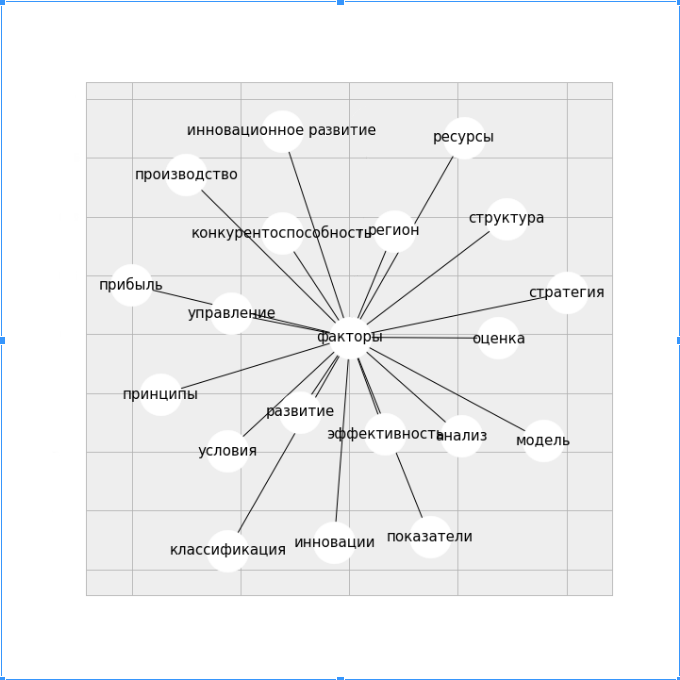
\includegraphics[width=1.0\linewidth]{Dissertation/pics/factory_sim} \\ а)
    \caption{Соседи вершины <<факторы>> в графе ключевых слов}
  \end{minipage}
  \hfill
  \begin{minipage}[ht]{0.49\linewidth}\centering
    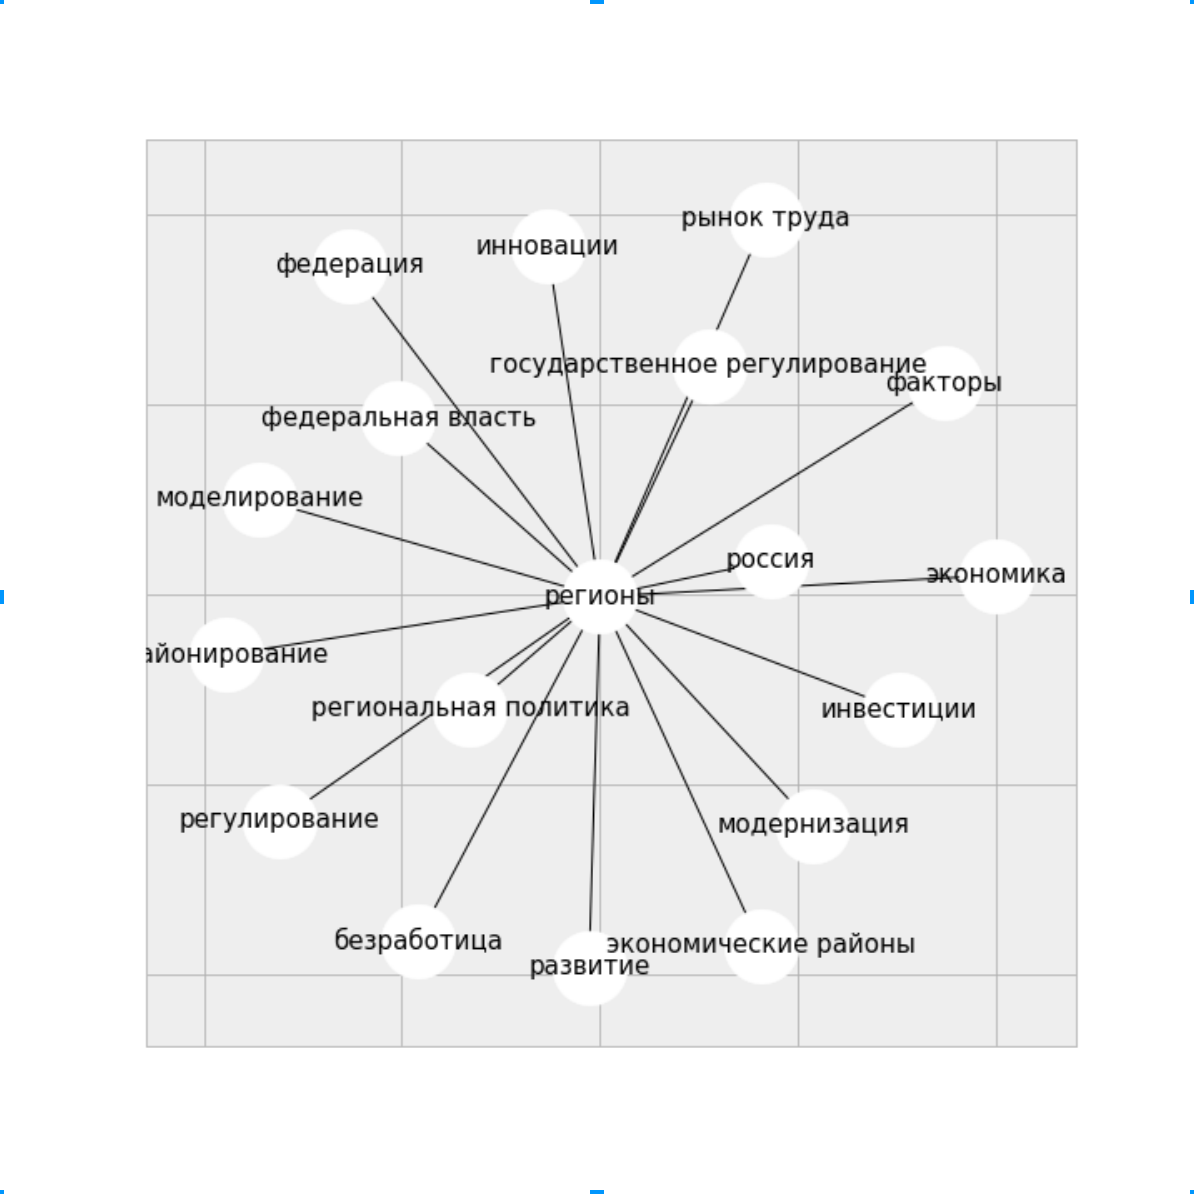
\includegraphics[width=1.0\linewidth]{Dissertation/pics/regiony_sim} \\ б)
    \caption{Соседи вершины <<регионы>> в графе ключевых слов}
  \end{minipage}
  \label{img:sim_1}
\end{figure}

На рисунках, представленных выше, видно, что графа ключевых слов не хватает для определения семантической близости пары слов. Легко заметить, что существуют связи, такие как <<факторы-модель>>, <<регионы-экономика>>, которые не обладают явной смысловой связью. Применение методов построения усеченного контекстного графа дает значительное улучшение качества классификации пар ключевых слов на семантически близкие и далекие. Далее указаны примеры найденных пар ключевых слов, близких по смыслу:

\textbf{β-адреноблокаторы   -   бета-адреноблокаторы}

\textbf{новые виды   -   новый вид}

\textbf{орви   -   острые респираторные вирусные инфекции}

\textbf{текущий уровень информационной безопасности   - политика информационной безопасности}

\textbf{умения   -   навыки}

\textbf{образное мышление   -   художественный вкус}

\textbf{хехцир   -   khekhtsyr}

\textbf{рынок банковских услуг   -   банковский рынок}

\textbf{тромболизис   -   тромболитическая терапия}

\textbf{параллельные алгоритмы   -   параллельное программирование}

\textbf{феминность   -   фемининность}

\textbf{полином  -  многочлен}

\textbf{корень  -   корни}

\textbf{primerun  -  примерун}

\textbf{fvk  -  fotovideoclub}

\textbf{еврореволюция  -   єврореволюція}

\textbf{silk\_plaster    -  шелковая\_штукатурка}.

\hl{Интересным в плане проводимых исследований является решение задачи определения похожих слов для заданного многозначного слова}. Рассмотрим семантически близкие понятия для слова <<орган>>.  В то время как в графе ключевых слов соседями для слова <<орган>> являются слова <<государство>>, <<сибирь>>, <<контроль>>, <<циркуляция>>, <<управление>>, в контекстном графе ближайшими являются слова <<музыковедение>>, <<организм>>, <<отклонение>>, <<делегирование полномочий>>, <<объект контроля>>. Легко заметить, что соседи в графе ключевых слов часто употребляются совместно со словом <<орган>>, однако определение таких отношений не вызывает затруднений. В случае контекстного графа были определены близкие по смыслу слова, при этом удалось восстанавить не только значение слова, связанное с юриспруденцией, но и близкие слова для значения из области музыки (<<музыковедение>>) и биологии (<<организм>>).

На рисунке \ref{img:sim_2} изображены несколько ближайших контекстно близких слов для слова <<студенты>> (отмечается, что полное множество соседей вершины слишком велико, чтобы его изобразить).

\begin{figure}[ht]
  \begin{minipage}[ht]{1.0\linewidth}\centering
    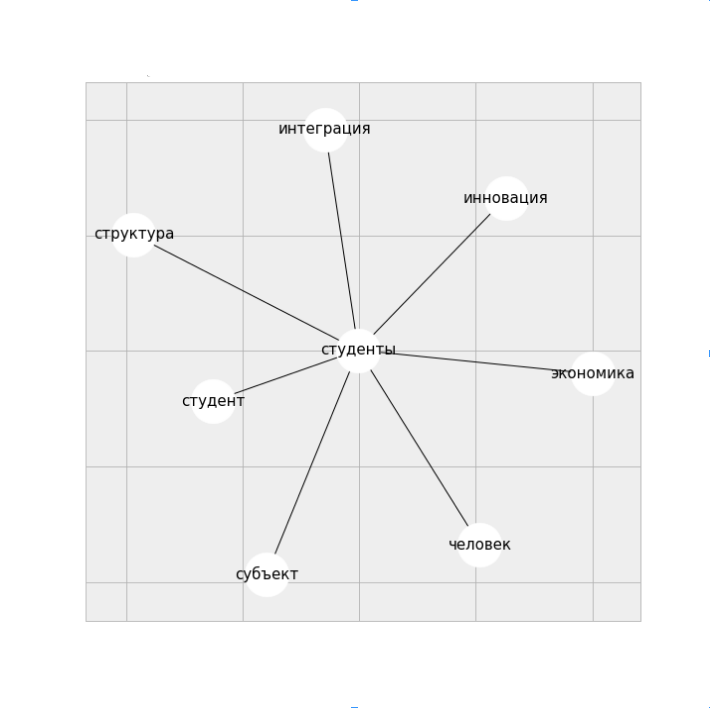
\includegraphics[width=1.0\linewidth]{Dissertation/pics/students_sim}
    \caption{наиболее близкие слова для слова <<студенты>> в контекстном графе}
    \label{img:sim_2}
  \end{minipage}
\end{figure}

\subsection{Выводы}
В настоящем разделе представлена разработанная автором модель семантической близости \emph{WordContSim}. Эта модель основывается на построении \emph{графа ключевых слов} и на идее о контекстной близости, детально описанной в разделе \ref{cont_sim}. Наряду с реализациями известных современных моделями семантической близости, программная реализация модели протестирована и по результатам сравнительного анализа продемонстрировано значительное улучшение уровня качества определения с ее помощью семантически близких пар на коллекциях наборов ключевых слов небольшого и среднего размеров. Процедура тестовой опробации описывается в разделе \ref{cont_sim_experiment}. \hl{Кроме этого, представлены примеры пар семантически близких ключевых слов для реальных коллекций ключевых слов. Эти примеры демонстрируют адекватность полученных результатов.}

К недостаткам разработанной модели можно отнести необходимость подбора правильных нормирующих множителей в формуле. Подбор формулы в общем случае может быть трудозатратной процедурой, поэтому были проведены исследования в направлении автоматического подбора формулы семантической близости по имеющейся графовой информации о ключевых словах и информационной системе. Результатом этих исследований стала модель, которая описывается далее в главе \ref{ml_sim}.

Отмечается практическая значимость полученных результатов в определении семантической близости ключевых слов. Кроме того, важной является возможность применения новой модели в других задачах информационного поиска и анализа данных, необходимых для функционирования аналитическо-информационных систем. Примером такой задачи является кластеризация множества ключевых слов, авторское решение которой описывается в разделе \ref{clustering}.

\section{Использование методов машинного обучения для улучшения модели близости слов. \hl{Модель \emph{WordMLSim}}} \label{ml_sim}

% >>> SYNOPSIS_2.3
В настоящем разделе рассматриваются методы улучшения качества определения семантической близости для пары ключевых слов с помощью методов машинного обучения с учителем. В тексте подробно описывается подход, который позволяет свести рассматриваемую задачу к задаче классификации, то есть к задаче определения целевой метки заданного объекта из заранее сформированного множества меток. Обучение с учителем подразумевают использование обучающей выборки - множества объектов, для которой известны истинные целевые метки. Эта выборка необходима для тренировки модели машинного обучения. С помощью обученной модели машинного обучения вычисляется предсказание целевой метки для произвольного объекта системы.

Сбор обучающего набора данных является обычно трудоемким процессом. Как правило, для его реализации требуется, как минимум, участие нескольких экспертов в предметной обласи, для которой собираются тренировочное множество. Более того, для некоторых задач, в число которых входит и задача определения семантической близости пар ключевых слов, является сложно даже правильно составить инструкцию для экспертов для адекватной оценки тестируемых примеров. Причина таких затруднений заключается в том, что семантическая близость - субъективная величина и сильно зависит от области применения, контекста, человека и задачи. Например, слово <<стол>> может быть близким по смыслу для слова <<стул>> из бытовых соображений. В то же время, если бы эти два слова были синонимами (а следовательно взаимозаменяемыми) в информационной системе, представляющей интернет-магазин, продающий мебель, имела бы место ситуация, когда пользователь ищет один из этих предметов, а в поисковой выдаче получает другой, что является недопустимым. Рассмотренные в следующих далее разделах алгоритмы сбора обучающего множества призваны разрешить обозначенные вопросы.

Автором настоящей диссертации были разработаны два автоматизированных метода формирования обучающих примеров без привлечения к этому процессу экспертов. Первый из них включает в себя набор эвристических алгоритмов создания обучающей выборки. Второй метод является полностью автоматическим и строится исключительно при помощи описанных в предыдущих главах графовых моделей представления данных. Важнейшим преимуществом этого метода является его универсальность и \hl{возможность его применимости} не только к задачам определения семантической близости, но и к любым другим задачам, в которых объекты системы представляются в виде некоторого графа и имеется необходимость в классификации отношений между парой объектов. Универсальность проявляется также в том, что выборка строится непосредственно по данным и не использует никакие внешние источники. \hl{Такой подход} позволяет определить отношения близости, специфичные для конкретной системы. Другое преимущество метода состоит в возможности использовать эффективные модели машинного обучения с учителем, вместо более слабых моделей без учителя, которые, \hl{к тому же представляют сложности при валидации} без обучающих примеров.
% SYNOPSIS_2.3 <<<

Задача классификации для определения семантической близости пары ключевых слов формулируется следующим образом. Пусть $X=\{x_i\}_{i=1}^N$ - множество пар ключевых слов. $x_i=(x^l,x^r)_i$ - пара ключевых слов, где $x_l,x_r$ - левое и правое слова из пары. $Y={0,1}$ - множество меток. Нулевое значение соответствует отсутствию семантической близости для пары ключевых слов, а единичное, напротив, сильной смысловой связи. Поскольку $Y$ состоит только из двух элементов, то такая задача является задачей бинарной классификации. $X^l=(x_i,y_i)_{i=1}^l$, где $x_i \in X, y_i \in Y$ - обучающающая выборка. Далее по обучающей выборке строится классификатор $a: X\rightarrow Y$

Процесс сбора обучающей информации является одним из важнейших этапов обучения эффективной модели определения семантической близости. Сложность этого процесса заключается в отсутствии возможности точно формализовать для пары ключевых слов отношения <<являются семантически близкими>> и <<не являются семантически близкими>>. Во многих случаях определение смысловой близости зависит от решаемой задачи, поэтому обучающие выборки для одной задачи могут не подходить для обучения моделей из другой. Например, пары ключевых слов <<математика>> и <<математическая статистика>> связаны отношением гиперонимии (<<математическая статистика>> является разделом <<математики>>), что влечет некоторую смысловую близость между понятиями. C другой стороны, если рассматривать задачу поиска документов системы по ключевым словам, то при заданном пользователем запросе <<информатизация, математика, вектор информатизации, информационные технологии, mathematica>>.  Для данного запроса ключевое слово <<математическая статистика>> не подходит по контексту данного запроса, кроме того, это ключевое слово является более узким по смыслу, чем <<математика>> и поэтому шансы пользователя получить релевантные запросу документы минимальны: если даже пользователь предполагал какую-то более узкую область, нет никаких оснований полагать, что это именно <<математическая статистика>>, а не, например, <<вычислительная математика>>. Обратная ситуация, когда пользователь ввел запрос <<математическая статистика, статистические тесты>>, то поиск в документах предположительно синонимичного слова <<математика>> также может привести к ухудшению выдачи. В результате этого действия, в выдачу вероятно попадут документы слишком общего смысла, такие как статьи про математику как науку.

Другим примером неоднозначности в определении семантической близости может служить различие в тематической направленности систем, в которых используются модели определения смысловой близости. Для наукометрических систем пара ключевых слов <<математическая статистика>> и <<вычислительная математика>> вряд ли должны иметь большое значение метрики смысловой близости, поскольку в рамках такой системы эти два понятия представляют два совершенно различных направления математики. В то же время, в системах более общей направленности, где могут присутствовать документы любого рода (а не только научные публикации), данная пара ключевых слов должна иметь более высокий уровень семантической похожести. Причина заключается в том, что для такой системы все термины относительно небольшого раздела <<математика>> могут считаться близкими по смыслу.

Качество модели определения семантической близости в данном случае целиком определяется двумя составляющими: параметрами обучающей выборки (качеством, разнообразием и количеством обучающих примеров) и эффективностью выбранного алгоритма машинного обучения. 

Лучшим алгоритмом для решения поставленной задачи бинарной классификации является модель градиентного бустинга на решающих деревьях XGBoost \cite{xgboost}. В ходе обучения происходит последовательное построение композиции решающих деревьев. Каждое следующее дерево стремится максимально уменьшить ошибку уже построенной части ансамбля. Анализ эффективности выбранной модели и \hl{результаты тестовых испытаний представлены в следующих далее подразделах.} 

\subsection{Методы формирования обучающей выборки} \label{art_train}
В данном подразделе описывается два разработанных способа получения обучающего набора данных. Первый из них использует различные эвристические идеи. Их суть состоит в том, как с помощью простых детерминированных процедур а, в некоторых случаях, внешних открытых наборов данных, получать примеры близких по смыслу пар ключевых. Такие методы имеют высокий уровень точности, однако слабое покрытие пространства пар ключевых слов системы. Второй способ заключается в использовании теоретико-графовых алгоритмов, способных выдавать примеры семантически близких и далеких пар объектов, основываясь на графовой структуре представления данных.

\subsubsection{Эвристические методы}
С позиции методологии различаются два типа алгоритмов сбора обучающей выборки. Первый из них заключается в использовании некоторых внешних словарей и дальнейшая фильтрация этих словарей по тем словам, которые присутствуют в информационной системе. Второй способ сначала использует некоторый генеративный алгоритм, \hl{а именно алгоритм}, который для заданного слова генерирует различные слова-кандидаты, потенциально близкие по смыслу к заданному. В качестве такого алгоритма может выступать, например, алгоритм, который в ходе работы для ключевого слова выбирает все слова, которые встретились с заданным внутри одного набора. Далее полученное множество фильтруется с помощью некоторого фильтрующего алгоритма. 

В результате работы программной реализации такого алгоритма определяются пары ключевых слов, которые принимаются за семантически близкие. Этот алгоритм должен обладать высокой точностью, хотя и возможно низкой полнотой определения семантической близости.  Другими словами, пары ключевых слов, объявленные семантически близкими, должны действительно являться похожими с вероятностью, близкой к 100\%. Следует однако отметить, что при этом количество таких пар может быть относительно невелико.

Примером такого алгоритма может быть алгоритм, считающий расстояние Левенштейна. Если редакторское расстояние не превосходит 1, то слова имеют очень схожее написание и  весьма вероятно, что они близки по смыслу. Такая процедура фильтрует значительную часть пар. Однако, те пары, которые прошли фильтрацию, почти всегда  имеют высокую степень смысловой близости. Таким образом каждый такой фильтр получает примеры близких по смыслу пар слов с высокой точностью, но низкой полнотой. Собранные с помощью такого подхода пары ключевых слов являются положительными примерами обучающей выборки для дальнейшего обучения.

В рамках исследований по теме настоящей диссертации автором были разработаны перечисленные далее эвристические методы сбора обучающей выборки.
\begin{itemize}
    \item Поиск простых аббревиатур. Ключевые слова системы разделяется на понятия, содержащие ровно одно слово - аббревиатуры, и понятия, содержащие более одного слова- расшифровки аббревиатур. Далее для каждого слова из множества аббревиатур и каждого словаиз множества расшифровок проверяется, действительно ли данная расшифровка является расшифровкой для данной аббревиатуры. Другими словами проверяется выполнение условия, что существуют такие префиксы слов расшифровки, которые могут полностью покрыть аббревиатуру. Если соответствие установлено, то пара аббревиатура-расшифровка добавляется в список пар-кандидатов. Далее к парам-кандидатам приписываются частоты входящих в них ключевых слов. Для каждой аббревиатуры берется не более 5 наиболее частотных вариантов расшифровок. Пары, прошедшие данную фильтрацию, формируют окончательное обучающее множество аббревиатур.
    \item Поиск скобочных аббревиатур. Иногда при написании ключевых слов-аббревиатур в скобках указывается правильная расшифровка для данной аббревиатуры. Такие действия позволяют собрать дополнительные пары аббревиатура-расшифровка для обогащения множества обучающих примеров.
    \item Поиск разных форм одного слова. С помощью пакета обработки естественного языка NLTK для каждого слова в системе рассматриваются различные его формы. Если одна из форм также присутствует в множестве всех ключевых слов, то пара слово-форма добавляется в обучающее множество.
    \item Поиск похожих по написанию слов. Рассматриваются все пары слов, расстояние левенштейна между которыми равно 1. Эти пары добавляются в обучающее множество.
    \item Поиск переводов с одного языка на другой. Данный метод использует API сервиса Яндекс.Переводчик и собирает варианты переводов ключевых слов с русского языка на английский.
    \item Поиск синонимов в тезаурусе WordNet. Были использованы пары синонимов и пары гипоним-гипероним. Кроме поиска по англоязычным синсетам был использован двухступенчатый подход определения синонимов: русскип слова переводились средствами сервиса Яндекс.Переводчик на английский язык, а затем поиск проводился уже по английским версиям слов.
    \item Использование открытых источников синонимов. Из словарей синонимов, доступных в сети Интернет, выделяются те пары, слова которых присутствуют в множестве ключевых слов.
\end{itemize}

Помеченные методы сбора данных позволяют собрать положительные примеры для обучения, то есть примеры пар ключевых слов, являющиеся семантически похожими. Однако для правильного обучения модели необходимы также и отрицательные примеры. С помощью небольших модификаций эвристических алгоритмов сбора положительных примеров можно получить алгоритмы для сбора отрицательных примеров. На этом направлении использованы следующие идеи.
\begin{itemize}
    \item Поиск антонимов в тезаурусе WordNet. Аналогично поиску синонимов был проведен поиск антонимов в базе WordNet. Также были использованы пары слов, расстояние в дереве WordNet между которыми превышает 2.
    \item Неправильные расшифровки для аббревиатур. Рассматриваются те аббревиатуры, для которых были найдены правильные расшифровки. Этим аббревиатурам ставятся в пару случайные многословные ключевые слова, которые точно не являются правильными расшифровками.
    \item Использование открытых источников антонимов.
    \item Случайные пары ключевых слов. Для каждого ключевого слова, для которого в выборке присутствуют положительные примеры, были взяты случайные ключевые слова в пару. На одно слово было сгенерировано не более, чем 10 пар. Данный метод был использован по следующим соображениям. Предполагается, что для каждого ключевого слова существует константное число близких по смыслу ключевых слов. То есть если в достаточно большой информационной системе начинает расти количество ключевых слов, то кол-во слов, похожих на данное слово, не будет расти линейно по числу уникальных слов системы. В то же время количество пар растет квадратично, а количество пар для заданного слова - линейно, а это означает, что если взять для заданного слова в пару случайное слово, то эта пара не будет связана семантически. При этом важным является подбор доли случайных пар. Если эта доля мала, то в выборке не будет достаточного разнообразия отрицательных примеров. Если же доля слишком велика, то случайные пары будут вносить слишком большой вклад в обучение модели. Это не является положительным фактором, потому что в случайные отрицательные пары не настолько качественны, как, например, антонимы из словаря. Оба этих случая приводят к ухудшению качества модели определения семантической близости.
\end{itemize}

В результате работы программных реализаций перечисленных выше алгоритмов было собрано 234974 положительных и 1175610 отрицательных примеров.

Обучение моделей на эвристически подобранных выборках имеет представленные далее заметные недостатки.

\begin{itemize}
    \item Смещение в данных. Для наилучшего обучения классификаторы необходимо, чтобы объекты обучающей выборки выбирались из распределения тех объектов, на которых классификатор будет работать в реальной системе. Рассмотрим данную особенность на следующем тривиальном примере. Допустим, что все пары ключевых слов системы делятся на Аббревиатуры (то есть пара аббревиатура - расшифровка аббревиатуры) и Переводы (слово на русском языке - его перевод на английский). Если Аббревиатур в системе 10\%, то и в обучающем подмножестве должно Аббревиатур должно быть 10\%. Если же аббревиатур при обучении будет значительно больше (например, 70\%), то модель начнет усиленно использовать те факторы, которые повышают ее качество на аббревиатурной части выборки, потому что это лучшим образом оптимизирует функцию потерь. Однако, в момент применения модели, к ней на вход будет поступать только 10\% аббревиатур и 90\% переводов и очень вероятно, что факторы, используемые моделью не будут оптимальны для классификации переводов и, тем самым, это улучшит качество реальных решаемых задач данным классификатором.  

        Другой недостаток смещения заключается в том, что если перегрузить обучающую выборку примерами неправильных переводов, то это негативно отражается на предсказанных уровнях близости во время этапа применения модели. Как следствие, это понизит средний уровень близости между переводами в системе. Отмеченное понижение приведет к тому, что если для данного ключевого слова (<<MSU>>) есть и правильная аббревиатура (<<Moscow State University>>), и правильный перевод (<<МГУ>>), то из-за рассмотренной манипуляции с обучающей выборкой, значимость перевода будет понижена. В конечном счете может оказаться, что согласно модели, все аббревиатуры лучше всех переводов. Такое поведение не очевидно и не основывается на реальной работе информационной системы. Такой сценарий возможен, поскольку положительные и отрицательные примеры берутся из разных источников. Поэтому степень покрытия ими всего разнообразия пар ключевых слов, а также возможность контролировать нужную долю положительных примеров остается под вопросом;
    \item Модель настраивается не под конкретную задачу и не под конкретные данные системы. Если, например, слова <<объединять>> и <<интегрировать>> попали в один внешний словарь синонимов общего назначения, то внутри информационной системы, направленной на изучение технических наук, эти слова определяют две различные математические операции. Может также случиться, что в узкоспециальных областях понятия могут являться слишком общими по смыслу, чтобы быть похожими. Примером такой пары может быть <<ураган>> и <<тайфун>>. Для пользователя, например, социальной сети эти слова действительно похожи. Однако, в рамках системы, изучающей различные природные явления, слова имеют важные смысловые отличия. Чем большей спецификой обладает тематика системы, тем четче прослеживается различия между словами, который с точки зрения словарей общей направленности, очень похожи.
    \item Сложность процесса сбора обучающей выборки. Для каждой системы нужны свои наборы эвристик, что затрудняет внедрение таких классификаторов повсеместно.
    \item Ошибки в выборке. По причине того, что частично выборка состоит из случайных примеров, весьма вероятно, что существует небольшое число пар, которые ошибочно промаркированы отрицательными. Это может понизить качество обученной модели. Помимо этого могут возникать ошибки второго рода. Например, если внешний сервис, предоставляющий переводы для слов и фраз допустил ошибку, то в множество положительных примеров попадет неправильный перевод для слова.
\end{itemize}

В связи с описанными выше недостатками, автором были проведены исследования возможности генерации обучающей выборки в автоматическом или полуавтоматическом режиме. Результаты этих исследований детально описаны в следующем далее подразделе.

\subsubsection{Алгоритм автоматизированной генерации обучающей выборки}
Для устранения недостатков, описанных в предыдущей подразделе, был разработан метод автоматической генерации обучающей выборки. Целью, как и ранее, является определение множества пар ключевых слов с соответствующими оценками  $((w_{i1}, w_{i2}), y_i)_{i=1}^{N}$, где $w_{ij} \in W$ - слова из множества всех ключевых слов информационно-аналитической системы, число $y_i \in {0, 1}$ указывает на то, близки ли семантически соответствующие слова (позитивные или положительные примеры) или нет (негативные или отрицательные примеры). Суть данного алгоритма заключается в использовании графовой структуры данных для получения обучающих примеров.

Рассмотрим алгоритм генерации обучающей выборки на упрощенном примере. Допустим, коллекция наборов ключевых слов $T$ состоит из приведенных далее наборов:

\textbf{[X, Y, W, A, C]}\

\textbf{[A, B, V, W]}\

\textbf{[A, C, Z, W]}\

\textbf{[C, Y, Z, W]}.\

Здесь каждая заглавная буква подразумевает одно ключевое слово. Различным буквам соответствуют различные ключевые слова. По этим данным имеется возможность построить граф ключевых слов $G_{kw}$, описание построение которого описывается в \ref{sect1_1}. Изображение этого графа приводится на рисунке \ref{img:art_train_graph}. 

\begin{figure}[ht]
  \begin{minipage}[ht]{1.0\linewidth}\centering
    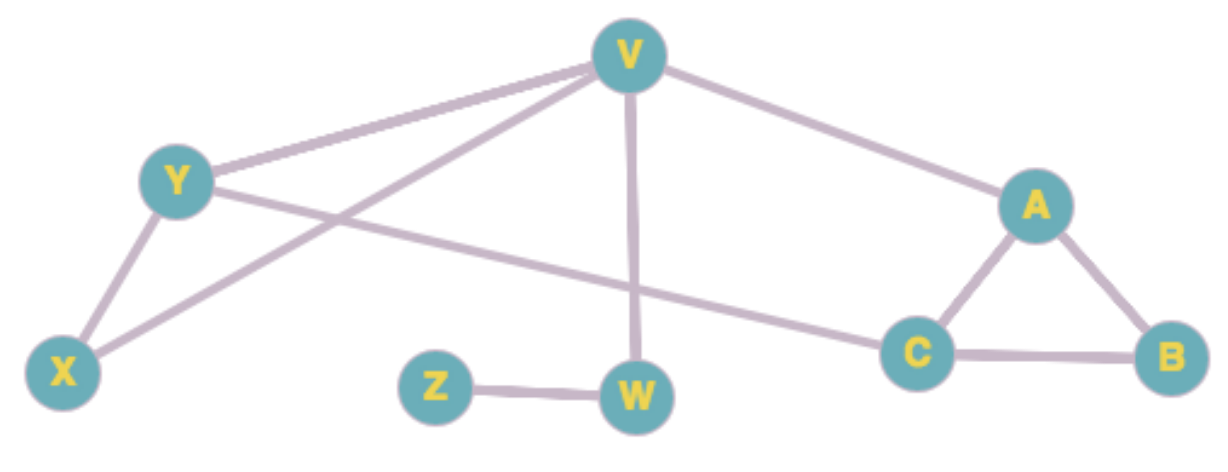
\includegraphics[width=0.7\linewidth]{Dissertation/pics/art_train_graph}
    \caption{Граф ключевых слов на упрощенной коллекции ключевых слов}
    \label{img:art_train_graph}
  \end{minipage}
\end{figure}

Для простоты изложения веса ребер на приведенной выше иллюстрации упускаются. Следующим шагом алгоритма является искусственная модификация исходной коллекции $T$. Для этого производятся следующие операции:
\begin{itemize}
    \item фиксируется дискретное распределение $P$;
    \item для каждого вхождения каждого слова коллекции $T$ из распределения $P$ выбирается случайное число $r$;
    \item если $r > 0$, то рассматриваемое вхождение слова $w$ заменяется на $w^{\ast r}$.
\end{itemize}

В программной реализации алгоритма генерации обучающей выборки для модификации ключевого слова к нему в конец добавляется специальный символ, который не используется в коллекции, с последующим добавлением номера $r$, выбранным случайно. Данный способ замены гарантирует уникальность нового ключевого слова среди множества ключевых слов $W$ изначальной коллекции $T$.

Рассматривая для упрощения в качестве дискретного распределения равномерное распределение из двух значений, исходная коллекция может быть модифицирована, например, следующим образом:

\textbf{[X, Y, W, $\mathbf{A_1}$, C]}\

\textbf{[A, $\mathbf{B_1}$, V, W]}\

\textbf{[$\mathbf{A_1}$, $\mathbf{C_1}$, Z, W]}\

\textbf{[C, Y, Z, W]}.\

Обозначим модифицированную коллекцию за $T^m$. После этого построим граф ключевых слов $G^{m}_{kw}$. Вид этого графа изображен на рисунке \ref{img:art_train_graph_m}.

\begin{figure}[ht]
  \begin{minipage}[ht]{1.0\linewidth}\centering
    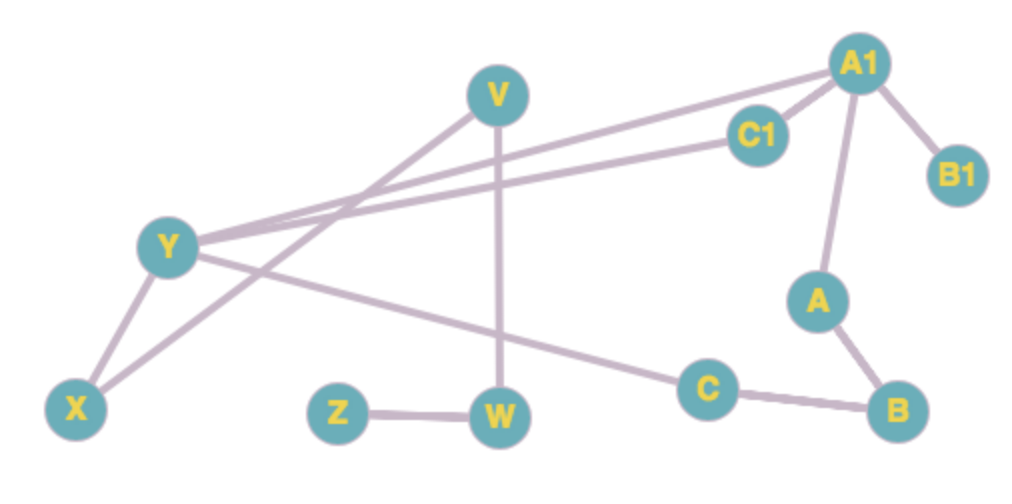
\includegraphics[width=0.7\linewidth]{Dissertation/pics/art_train_graph_m}
    \caption{Граф ключевых слов на модифицированной упрощенной коллекции ключевых слов}
    \label{img:art_train_graph_m}
  \end{minipage}
\end{figure}

\hl{Можно заметить, что в ходе работы алгоритма были модификацированы вершины $A, B$ и $C$. После такого перестроения, в графе появились соответствующие им вершины $A_1, B_1$ и $C_1$. Однако, эти пары не обязаны соединяться ребром в этом графе.}

В процессе модификации семантическому изменению слова не подверглись, поскольку к ним, фактически, были приписаны служебные символы в конец.  Другими словами, пара слов $(A, A_1)$ является, по сути, одним и тем же словом, и, следовательно, может быть положительным обучающим примеров для выборки, потому что для этих слов существует две вершины в графе. Таким образом, для рассмотренного примера определены положительные обучающие примеры $(A, A_1), (B, B_1), (C, C_1)$. 

Задачей машинного обучения в данном случае является восстановления факта идентичности различных версий одного слова путем выявления различных графовых связей между парами обучающих примеров. Под графовыми связями здесь и далее подразумевается различные меры и характеристики, которые можно вычислить для пары вершин одного графа. Такими характеристиками являются длины кратчайших путей, количество общих соседей между вершинами, факт принадлежности одной компоненте связности и прочее. Далее используется предположение о том, что найденные закономерности, влияющие на значение уровня семантической близости в графе $G^{m}_{kw}$, также имеют место быть в графе $G_{kw}$. Это предположение имеет место по той причине, что графы $G^{m}_{kw}$ и $G_{kw}$ строятся при помощи одного и того же алгоритма.

Важную роль в разработанном алгоритме генерации выборки играет распределение, из которого берутся индексы модифицированных объектов. Использование бернуллиевского распределения  с вероятностью успеха $p=0.5$ имеет существенный недостаток. Этот недостаток состоит в том, что ключевые слова $w$ и $w_1$ будут встречаться примерно одинаковое количество раз в коллекции $T^m$. Таким образом, обученная модель будет предполагать, что пара хороших синонимов в исходной коллекции $T^m$ также обладает этим свойством, что неверно. Проиллюстрировать это можно следующим примером. Пара слов <<жалованье>>, <<зарплата>> являются синонимами, однако очевидно, что слово <<жалованье>> является устаревшим и в наше время употребляется значительно реже. 

В связи с приведенными замечаниями, для исследований было выбрано более сложное распределение: геометрическое распределение. Такое распределение помогает преодолеть недостаток, описанный ранее. Кроме того, засчет бесконечного носителя это распределение позволяет генерировать множество различных вариаций для одного слова (количество различных вариаций для одного слова ограничено числом употреблений исходного слова в коллекции $T$). Этот факт является важным достоинством этого распределения по двум причинам. Во-первых, такое положение дел более приближено к реальности, потому что ключевое слово может иметь более, чем одно близкое по смыслу слово. Во-вторых, это распределение позволяет существенно обогатить выборку, поскольку любую пару модификаций исходного слова можно считать положительным примером для обучения. Плотность геометрического распределения в зависимости от вероятности успеха $p$ изображена на рисунке\ref{img:geom_distr}. На рисунке \ref{img:geom_distr_2} показана гистограмма индексов при генерации модифицированных версий некоторого ключевого слова.

\begin{figure}[ht]
  \begin{minipage}[ht]{1.0\linewidth}\centering
    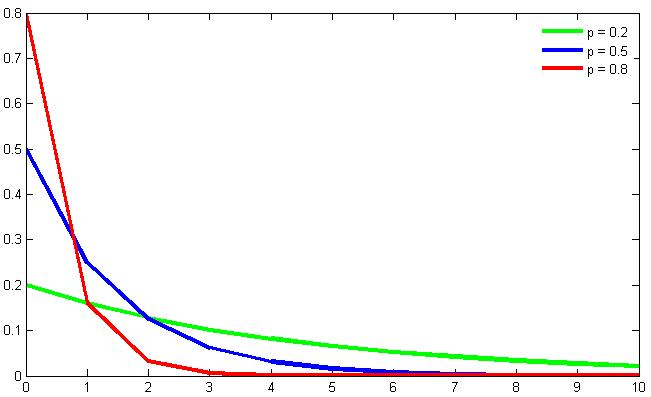
\includegraphics[width=0.7\linewidth]{Dissertation/pics/geom_distr}
    \caption{Плотность геометрического распределения при разных значениях}
    \label{img:geom_distr}
  \end{minipage}
\end{figure}

\begin{figure}[ht]
  \begin{minipage}[ht]{1.0\linewidth}\centering
    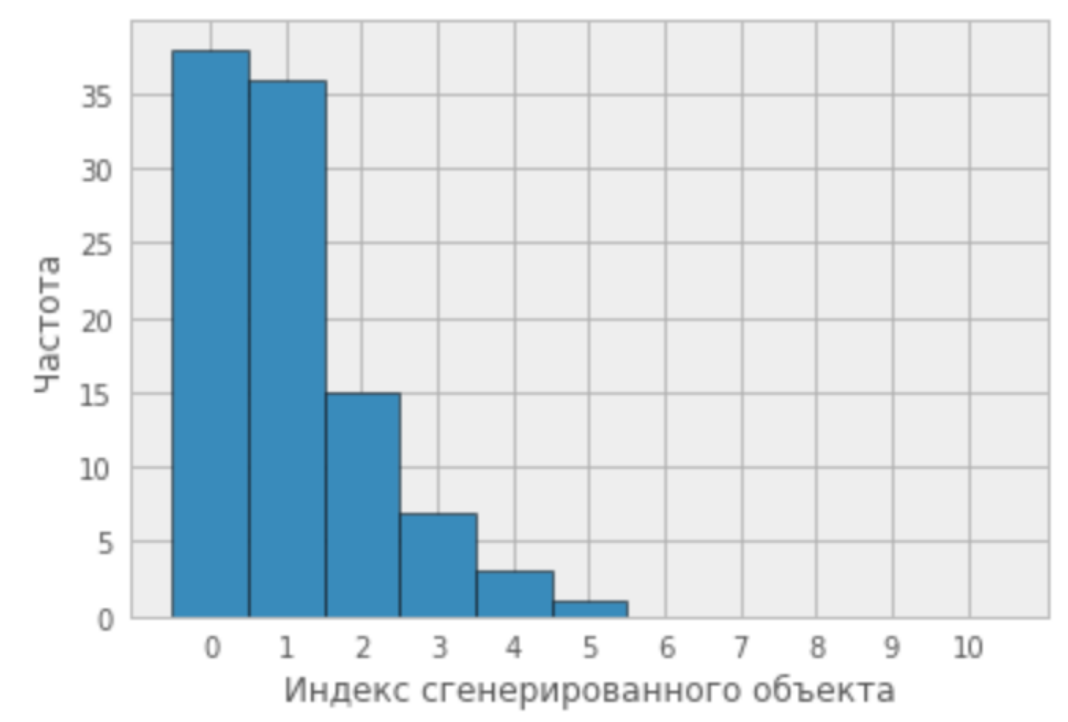
\includegraphics[width=0.7\linewidth]{Dissertation/pics/geom_distr_2}
    \caption{Зависимость количества объектов от сгенерированного индекса}
    \label{img:geom_distr_2}
  \end{minipage}
\end{figure}

После того, как положительные примеры обучающей выборки собраны, необходимо создать также и отрицательные примеры. Для отрицательных примеров используется следующий алгоритм:
\begin{enumerate}
    \item построение графа ключевых слов $\hat{G}$ по модифицированному множеству ключевых слов;
    \item для каждого слова $w$, попавшего в множество пар положительных примеров, рассматриваются случайные $k$ соседей $v_1, v_2, ..., v_k$ на расстоянии $2$ в графе $\hat{G}$;
    \item все пары $(w, v_i)_{i=1}^k$ принимаются отрицательными примерами.
\end{enumerate}

Мотивация для использования этого алгоритма заключается в следующем. Для обучения модели отрицательные примеры должны быть содержательными. Если рассмотреть абсолютно случайные пары ключевых слов, то большинство полученных примеров не будут представлять особой значимости для модели. Причина в том, что большинство статистических характеристик в этом случае будут иметь нулевое или близкое к нему значение. Между случайными вершинами в графе может не быть путей, они могут не иметь общих соседей, могут быть расположены на слишком большом удалении друг от друга и т.д.. Такие случайные пары не дают никакой информации для модели для более сложных случаев, когда слова находятся достаточно близко друг к другу в графе, но при это не являются семантически близкими. Однако, именно такие случаи и представляют интерес в рамках решаемой задачи.

С другой стороны, если для заданного ключевого слова в качестве отрицательных примеров брать непосредственных соседей в графе (то есть максимально близкие вершины), то слишком часто будут появляться пары, которые в действительности близки по смыслу. Это происходит потому, что среди слов одного набора могут встречаться похожие слова. Вследствие этого, среди отрицательных примеров будет большое число примеров, которые ошибочно были промаркированы отрицательными, что не позволит качественно обучить модель.

Поэтому соседи вершины на расстоянии два представляется наиболее подходящим компромиссом: среди них не так часто встречаются семантически близкие пары, однако при этом они несут в себе содержательный сигнал, на котором можно эффективно обучаться. С учетом изложенных выше соображений, алгоритм автоматизированной генерации обучающей выборки выгляди следующим образом.

\begin{itemize}
    \item Входные параметры: $N$, $p$, $k$, $D$.
    \item Для каждого набора ключевых слов $t \in T$ системы $D$:
        \begin{itemize}
            \item для каждого \textit{вхождения} ключевого слова $w$:
                \begin{itemize}
                    \item если количество вхождений в коллекцию превосходит пороговое значение $N$:
                        \begin{itemize}
                            \item из геометрического распределения с параметром $p$ выбирается число;
                            \item вхождение ключевого слова $w$ заменяется $w_p$;
                            \item слово $w_p$ заносится в список модификаций для слова $w$.
                        \end{itemize}
                    \item иначе
                        \begin{itemize}
                            \item вхождение ключевого слова $w$ не изменяетсязаменяется $w_0$.
                        \end{itemize}
                \end{itemize}
            \item модифицированная версия набора ключевых слов добавляется в множество $D^{m}$
        \end{itemize}
    \item Для каждого уникального ключевого слова $w \in W$:
        \begin{itemize}
            \item каждую пару модификаций $(w_i, w_j)$ ключевого слова $w$ добавить в обучающее множество $X_{train}$ в качестве положительного примера.
        \end{itemize}
    \item Для модифицированной версии коллекции наборов ключевых слов $D^{m}$ произвести построение графа ключевых слов $G^m_{kw}$.
    \item Для каждой вершины $w_i$ из множества модифицированных вершин графа $G^m_{kw}$:
        \begin{itemize}
            \item выделить множество  $G^m_{kw, 2}(w_i) = neigbors(G^{m}_{kw}, w_i, 2)$ соседей вершины $w_i$ в графе $G^{m}_{kw}$ на расстоянии $2$;
            \item из множества $G_{2}(w_i)$ выбрать случайно $k$ вершин $v_1, ... v_k$ и для каждой вершины добавить пару $(w_i, v_j)$ в $X_{train}$ в качестве отрицательного примера.
        \end{itemize}
    \item Вернуть обучающее множество $X_{train}$, граф $G^{m}_{kw}$.
\end{itemize}

Значения параметров $N$, $p$, $k$ были определены как $10$, $0.9$, $5$, соответственно. Необходимость выбора параметра $N$ обусловлена тем наблюдением, что если слово встречается в коллекции $D$ слишком редко, то всего его модификации будут встречаться в коллекции $D^m$ еще реже. Для этих слов в графах будет мало связей. Поэтому те слова $w$, которые встретились в исходной коллекции меньше, чем $N$ раз, игнорируются алгоритмов, а точнее, всегда заменяются на $w_0$.

Вхождением ключевого слова в описанном выше алгоритме является появление ключевого слова в одном конкретном наборе ключевых слов. Поскольку одно слово может присутствовать во многих наборах, то число вхождений равно количеству наборов, содержащих данное ключевое слово.

Следующее далее утверждение дает оценку вычислительной сложности алгоритма генерации обучающей выборки.

\textbf{Утверждение 5.} Расчет искусственной обучающей выборки имеет сложность $O(f^2 * k + w^2 * k^2)$, где $f$ - максимальная частотность слова в коллекции, $k$ - количество уникальных слов в коллекции, $w$ - максимальный размер набора в коллекции ключевых слов.

%Процедура $m$ - максималь
%кол-во уникальных k
%кол-во наборов m
%максимальное число слов в наборе w
%максимальная частотность слова в коллекции f
%w * m - прошли по наборам, модиф кл слова.
%
%f * k - все наборы, один раз прошлись
%f^2 - модификаций для одного слова
%f^2 * k - для всех
%f * k - построение графа
%k - максимальный размер набора (все уникальные слова попали в один набор)
%k * k  (http://www.cs.tau.ac.il/~zwick/papers/sparse.pdf умножение matr n*n -> m*n , m=nnz)
% http://www.stat.ucdavis.edu/~chohsieh/teaching/ECS289G_Fall2015/complexity.pdf
%f^2 * k + k^2

\textbf{Лемма 1.} Построение положительных примеров искусственной обучающей выборки имеет сложность $O(f^2 * k)$, где $f$ - максимальная частотность слова в коллекции, $k$ - количество уникальных слов в коллекции.

\textbf{Доказательство.} 
Число всех ключевых слов системы с повторениями не превышает значение $f * k$. Необходимо пройти один раз по всем ключевым словам коллекции, чтобы сгенерировать для них модифицированную версию - это требует $O(f * k)$ операций. При этом полагается, что выбор случайного числа из выбранного распределения занимает константное время. Следующим шагом необходимо из модифицированных версий каждого слова получить всевозможные пары. Для каждого из $k$ слов может быть получено не более, чем $f$ модификаций слова, поскольку каждая модификация была получена из некоторого исходного слова, которое в свою очередь было использовано не более, чем $f$ раз в коллекции. Для генерации всех пар для данного исходного слова необходимо $O(f^2)$ времени, а для всех уникальных слов - $O(k * f^2)$.

\textbf{Лемма 2.} Построение отрицательных примеров искусственной обучающей выборки имеет сложность $O(w^2 * k^2)$, $k$ - количество уникальных слов в коллекции, $w$ - максимальный размер набора в коллекции ключевых слов.

\textbf{Доказательство.} 
. Построение графа ключевых слов занимает не более $O(k^2)$ времени. Далее необходимо рассчитать соседей для каждой вершины на расстоянии $2$. Для этого необходимо возвести в квадрат матрицу смежности графа. При хранении графа в виде разреженной матрицы, операция умножения матрицы размера $(k*k)$ на себя требует $O(nnz * k)$ операций, где $nnz$ - количество ненулевых элементов. Поскольку в графе ключевых слов ребрами являются те пары ключевых слов, которые входят в один набор, то количество ребер в графе, как и количество ненулевых элементов в матрице смежности, не превышает $O(w^2 * k)$, то сложность поиска соседей второго порядка будет равна $O(w^2 * k^2)$. Предполагая, что операция взятия случайного числа из заданного распределения занимает константное время, получаем, что генерация отрицательных примеров для искусственной обучающей выборке требует $O(w^2 * k^2)$ операций.

Из двух доказанных выше лемм следует утверждение 5. После того, как обучающие выборки созданы, необходимо для обучающих объектов посчитать различные графовые характеристики, которые будут описывать данный объект. Вместе с целевой переменной эти характеристики необходимы для обучения классифицирующей модели.

Разработанный подход к определению смысловой близости с помощью машинного обучения и автоматизированной обучающей выборки обладает следующей особенностью. Обученная на графе $G^m_{kw}$ модель впоследствии используется для предсказания семантически близких пар уже на графе $G_{kw}$. Это накладывает некоторые ограничения на признаки, которыми описываются объекты машинного обучения. В следующем разделе приводится описание этих признаков и объясняется отмеченная особенность.

%\begin{Алгоритмо
\subsection{Признаковое описание модели машинного обучения} \label{sec:features}
Под признаковым описанием пары ключевых слов понимается определение набора функций, вычисляющих некоторые числовые характеристики для рассматриваемых слов. Такие функции (факторы) могут использовать оба слова в явном виде (расстояние Левенштейна, количество общих слов и т.д.) или только одно из слов (частотность данного слова в корпусе, количество символов в слове и т.д.), что порождает пару значений признака для левого и правого слов из пары. 

\hl{Результатом применения программных реализаций функций к паре ключевых слов является фиксированный по длине массив чисел. Массивы чисел, посчитанные для всех пар ключевых слов обучающей выборки, образуют так называемую матрицу \emph{объектов-признаков}. Строки этой матрицы представляют собой признаковое описание обучающих объектов выборки, а столбцы соответствуют признакам. }

\hl{Признаком может являться любая функция, способная вычислить значение для поданного на вход объекта. Cледует однако понимать, что не каждая функция может быть полезна в процессе обучения. Формирование списка признаков, наилучшим образом характеризующих объекты, является важным шагом при решении задачи машинного обучения с использованием модели градиентного бустинга. Массив признаков представляет собой то, как <<видит>> объект модель машинного обучения. В связи с этим, признаки должны в полной мере описывать объект. В рамках поставленной задачи это означает, что для пары ключевых слов полезными могут быть признаки, описывающие различные синтаксические, морфологические, семантические, статистические и графовые характеристики пары рассматриваемых слов.}

\hl{Таким образом, в ходе работы алгоритма для всех рассматриваемых пар ключевых слов происходит вычисление всего набора факторов. В результате появляется матрица объект-признак. Строка этой матрицы является описанием конкретной пары ключевых слов, а столбец определяет значения некоторого признака для все пар. Для обучающей выборки кроме матрицы объект-признак также имеется вектор-столбец истинных значений. Это позволяет обучать алгоритмы машинного обучения, после чего применять обученные модели для предсказания на новых данных (для которых также можно получить признакое описание).}
\hl{ Является важным отметить тот факт, что описанные в предыдущем подразделе методы формирования обучающей выборки вносят существенные ограничения на разработку признаков. В рамках данной работы выыделяется два принципиально различных класса признаков: \emph{графовые} и \emph{языковые}. }

\hl{Графовыми факторами являются те, которые возможно получить по графам, описанным в предыдущих главах. Графовые признаки ни в каком виде не учитывают содержимое вершин графа, то есть не учитывают особенности ключевого слова с точки зрения естественного языка. Вместо этого, такие признаки используют только связи данной вершины с другими вершинами.}

\hl{Языковые признаки, напротив, используют знания из области обработки естественного языка: морфологические, синтаксические и семантические. Кроме того, к классу языковых были отнесены признаки, вычисленные при помощи внешних по отношению к рассматриваемой информационно-аналитической системы наборов данных.}

\hl{Необходимость выбранного разделения признаков на классы обусловлена следующим обстоятельством.} В связи с особенностями процесса формирования автоматизированной обучающей выборки, для моделей, обученных на этом типе выборки не представляется возможным использование языковых факторов. Причиной этому является принцип построения автоматизированной обучающей выборки. Для генерации нового позитивного примера к рассматриваемому слову приписывается служебный, семантически незначащий суффикс. Это означает, что языковые различия между словами в такой паре является искуственными  и не отражают действительную природу вещей. \hl{Использование эвристической обучающей выборки не накладывает ограничений на выбор признаков, однако обладает недостатками, описанными в предыдущем подразделе.}

\hl{После вычисления значений всех признаков начинается процесс обучения модели. Для его запуска необходимо подать матрицу объектов-признаков и обучающую выборку (эвристическую или автоматизированную) на вход модели обучения. С учетом изложенных выше соображений, для решения поставленной задачи необходимо определить множество факторов, которое позволит достичь наилучшего показателя качества модели машинного обучения. Для автоматизированной выборки выделяются графовые факторы, а для эвриcтической - графовые и языковые. Особый интерес представляет автоматизированная выборка, поскольку ее использование позволяет полностью автоматизировать весь процесс решения задачи семантической близости пары ключевых слов.}

\hl{Полный список рассмотренных признаков приводится в следующей далее таблице \ref{tbl:features}}.


%\begin{tabularx}{10cm}{|p{4cm}|p{4cm}|p{2cm}|}
%\begin{table}[htb]
%\tiny    
\begin{longtable}{|p{5cm}|p{4cm}|p{5cm}|}
        \hline
        Признак & Описание & Тип \\ \hline
        Расстояние в графе ключевых слов & & Парный \\ \hline
        Расстояние в усеченном контекстном графе ключевых слов & & Парный/графовый \\ \hline
        Контекстная близость & Вариации контекстной близости, описанные в подразделе \ref{cont_sim} & Парный/графовый \\ \hline
        Ранк контекстной близости & & Парный/графовый \\ \hline
        Мера абстрактности & Мера общности понятия, описанная в разделе \ref{abstractness} & Одиночный/графовый \\ \hline
        Количество вершин в кластере & Количество вершин кластера для рассматриваемой вершины & Одиночный/графовый \\ \hline
        PageRank вершины графа & Значение PageRank меры для вершин графов & Одиночный/графовый \\ \hline
        EdgeRank ребра графа & Значение EdgeRank меры для ребер графов & Парный/графовый \\ \hline
        Вес ребра в графе ключевых слов & & Парный/графовый \\ \hline
        Частотность левого слова & & Одиночный/графовый \\ \hline
        Частотность правого слова & & Одиночный/графовый \\ \hline
        Совместная частотность в корпусе & & Парный/графовый \\ \hline
        Pointwise mutual information & & Парный/графовый \\ \hline
        Мера Жаккара & Считается по вершинам соседям & Парный/графовый \\ \hline
        Число простых путей в графах между вершинами & Считается по обоим графам & Парный/графовый \\ \hline
        Betweenness centrality  & & Одиночный/графовый \\ \hline
        Closeness centrality & & Одиночный/графовый \\ \hline
        Eigen vector centrality & & Одиночный/графовый \\ \hline
        Значение потока между вершинами & & Парный/графовый \\ \hline
        Количество соседей & На расстоянии 1 и 2 (два фактора) & Одиночный/графовый \\ \hline
        Количество общих соседей & На расстоянии 1 и 2 (два фактора) & Парный/графовый \\ \hline
        Расстояние Левенштейна & & Парный/языковой \\ \hline
        Часть речи слова & Категориальный признак & Одиночный/языковой \\ \hline
        Количество слов  & & Одиночный/языковой \\ \hline
        Количество букв & & Одиночный/языковой \\ \hline
        Количество общих слов & & Парный/языковой \\ \hline
        Пословная мера Жаккара & & Парный/языковой \\ \hline
        Нграммная мера Жаккара & Используется биграмное и триграмное представление слов & Парный/языковой \\ \hline
        Пара слов на разных языках & Бинарный признак & Парный/языковой \\ \hline
        Одно слово является аббревиатурой/сокращением  для другого & Бинарный признак & Парный/языковой \\ \hline
        Одно слово является формой другого & Бинарный признак & Парный/языковой \\ \hline
        Одно слово является транслитерацией другого & Бинарный признак, использован наивный алгоритм транслитерации & Парный/языковой \\ \hline
        Расстояние по дереву WordNet & & Парный/языковой \\ \hline
        Глубина слова в дереве WordNet & & Одиночный/языковой \\ \hline
        Косинусное расстояние между word2vec представлениями слов & & Парный/языковой \\ \hline
        Средняя частотность слов в корпусе & В качестве слов рассматриваются не ключевые слова, а отдельные слова естественного языка  & Одиночный/языковой \\ \hline
        Косинусное расстояние пословных TFIDF представлений & В качестве слов рассматриваются не ключевые слова, а отдельные слова естественного языка & Парный/языковой \\ \hline
        Косинусное расстояние нграммных TFIDF представлений & Подсчитано на символьных триграммах & Парный/языковой \\ \hline

\caption{Факторы, используемые моделью для обучения} \label{tbl:features}
\end{longtable}
%\end{table}


В таблице \ref{tbl:features} представлен набор факторов, который был использован в работе для обучения модели. 


Заключительным этапом в построении классификатора является процесс настройки его параметров. Данная процедура реализуется с помощью стандартной схемы подбора. Суть ее заключается в следующем.

\begin{enumerate}
    \item \textbf{Выбирается набор параметров модели.}
    \item \textbf{Производится разбиение обучающей выборки на несколько подмножеств.} В исследованиях использовалось 5 подмножеств. В каждое подмножество входило приблизительно $20\%$, причем для всех пар ключевых слов обучающей выборки выполняется, что если слово $w_i$ находится в одном из подмножеств, то и все пары $\{(w_i, w_j) | (w_i, w_j) \in X_{train}\}$ также лежат в этом подмножестве.
    \item \textbf{Производится обучение модели.} Модель обучается на 4 подмножествах из 5, используя набор входных параметров.
    \item \textbf{С помощью обученной модели вычисляются предсказания уровня семантической близости.} Предсказание происходит на оставшемся пятом подмножестве обучающей выборки. Такая схема тестирование носит название перекрестной валидации.
    \item \textbf{Вычисляется значение оптимизируемой метрики}. Предсказание происходит на оставшемся пятом подмножестве обучающей выборки. Такая схема тестирование носит название перекрестной валидации.
    \item \textbf{Шаги 3-5 повторяются для всех возможных сочетаний подмножеств по 4.} Значение метрики усредняется.
    \item \textbf{Шаги 1-6 повторяются для всех рассматриваемых наборов параметров.} В ходе работы запоминается тот набор параметров, на котором достигается наилучшее значение метрики.
    \item \textbf{Обучается финальная модель.} Для этого используются оптимальные параметры, найденные на шаге 7. Для обучения используется вся обучающая выборка.
\end{enumerate}

Обучив модель, появляется возможность с ее помощью предсказывать значения уровня близости для любой пары ключевых слов коллекции $D$. В следующем разделе описываются тестовые испытания программных реализаций представленных моделей.

%Основную идею можно описать следующим образом. Для решения задачи выбирается множество пар ключевых слов, которые являются близкими по смыслу, а также множество пар, которые напротив, далеки друг от друга по смыслу. Эти два множества вместе составляют обучающую выборку или разметку. Способы получения обучающих выборок были описаны в предыдущих разделах. Следующим шагом выбирается метрика (т.н. функция потерь), которую алгоритм будет оптимизировать в ходе обучения. К данной задаче применительны как функции потерь для задач классификации (например, логарифмическая функция потерь), так и функции потерь для задач регрессии (такие как среднеквадратичная ошибка). Несмотря на то, что первое семейство метрик более естественно для решаемой  задачи (поскольку решается задача бинарной классификации: является ли пара ключевых слов близкой по смыслу или нет), по результатом экспериментов, рассмотрение задачи определения семантической близости как задачи регрессии может даже более качественный результат. Далее выбирается алгоритм машинного обучения, на вход которому подается признаковое описание элементов обучающей выборки, а также истинные ответы для объектов этой обучающей выборки. Множество признаков детально описано в разделе \ref{sec:features}. В рамках рассматриваемой задачи наилучшее качество продемонстрировала реализация алгоритма градиентного бустинга на решающих деревьях XGBoost. Отмечается, что обучение алгоритмов также непрерывно связано с настройкой гиперпараметров, но в данном случае это значительно более простая задача, поскольку для конкретного алгоритма машинного обучения есть набор рекомендаций по настройке параметров. Также существует программные комплексы, способные настроить гиперпараметры в автоматическом режиме. После того, как модель обучена, можно применять её к произвольным парам ключевых слов, предварительно посчитав для них их признаковое описание. На выходе будет степень уверенности модели в том, что пара слов является семантически похожими понятиями.

\subsection{Тестовые испытания}
\hl{Далее представлены результаты тестирования программных реализаций описанных алгоритмов определения близости с использованием методов машинного обучения. Рассмотрены два способа проведения тестовых испытаний: на отложенной части обучающей выборки и на множестве пар одинаковых слов.}

\hl{Тестирование разработанных программных реализаций моделей необходимо в связи с их практической важностью для интеллектуально-аналитических систем. Описанные ранее модели используются в дальнейшем для определения уровня семантической близости наборов ключевых слов, а также для решения прикладных задач, описание которых приводится в главе \ref{chapt_applications}. }

\textbf{Тестирование обучения модели с автоматизированной выборкой.}
Тестирование программных реализаций алгоритмов проводилось на следующих наборах данных.
\begin{itemize}
    \item \textbf{Aminer}\footnote{https://www.aminer.cn/oag2019}. Открытая коллекция наукометрических данных, созданная авторами \cite{aminer}. Коллекция располагает англоязычной информацией о научных публикациях, авторах, конференциях и ключевых словах к научным статьям. Для тестирования были выбрана коллекция ключевых слов из категории \emph{обработки естественного языка} (\emph{natural language processing}).
    \item \textbf{KeywordsRu}. Коллекция наборов русскоязычных ключевых слов, собранных из сети Интернет. Используемая выборка была использована ранее в разделе \ref{cont_sim_experiment}.
    \item \textbf{KeywordsEn}. Коллекция наборов русскоязычных ключевых слов, собранных из сети Интернет. Ключевые слова для данной выборки были собраны аналогично процедуре сбора русскоязычного набора данных \emph{KeywordsRu}.
\end{itemize}

\hl{Валидация качества работы программных реализаций алгоритмов была проведена с помощью эвристической обучающей выборки, представленной в предыдущем подразделе. Модели на вход подается одна из рассматриваемых коллекций ключевых слов. Программная реализация строит все необходимые графы ключевых слов, определяет на их основе автоматизированную обучающую выборку и вычисляет факторы для каждого элемента выборки. Далее запускается процесс обучения модели. После чего происходит процесс применения обученной модели к объектом эвристической обучающей выборки. Последним этапом является вычисление значения метрик, характеризующих качество работы программной реализации.} 

\hl{Кроме того, для рассматриваемых коллекций ключевых слов используются известные модели вычисления семантической близости. В рамках этого эксперимента были выбраны уже представленная ранее модель \emph{Word2Vec}, а также модель \emph{Node2Vec} (\cite{node2vec}). В то время, как Word2Vec использует знания о языке для решения задачи семантической близости, модель Node2Vec определяет близость между вершинами графа. Для этого исследователя определяют векторное представление для вершин графа. Меньшее расстояние между векторами влечет более выраженную структурную связь между соответствующими вершинами. Следует также отметить, что модель Node2Vec переносит идеи, заложенные в модель Word3Vec, с текстовых данных на графовые.}

\hl{Выбор моделей Word2Vec и Node2Vec для сравнения c моделью, представленной в данном разделе, обусловлен следующими соображениями. В первую очередь, было необходимо продемонстрировать высокий уровень определения семантической близости между словами естественного языка. Для этой цели авторская модель сравнивается с зарекомендовавшим в индустрии решением - моделью Word2Vec. Кроме этого, поскольку в ходе работы используются графовые методы определения близости, является важным сравнить реализацию модели с известными решениями вычисления близости между вершинами графа. В качестве такого решения выступает модель Node2Vec.}

\hl{В дополнении к этому, представляет интерес следующее рассуждение. Как было показано ранее в подразделе \ref{features}, разработанные признаки являются функциями от пары вершин графа и, следовательно, каждый признак может представлять некоторую меру близости пары ключевых слов. Подобно этому модель \emph{WordContSim}, с одной стороны, является признаком для модели \emph{WordMLSim}, а с другой, оказывается самодостаточным подходом к определению смысловой близости, как было показано ранее в разделе \ref{wordcontsim}. В этой связи важно проверить, что модель, обученная на всем множестве факторов, качественно превосходит любой из признаков, входящих в ее состав. Этот факт докажет целесообразность применения машинного обучения в рамках поставленной задачи.}

\hl{В следующей далее таблице \ref{tbl:sim_res} представлены результаты тестирования программной реализации модели \emph{WordMLSim}.}


\begin{table}[htb]
\begin{tabular}{|l|l|l|l|l|l|l|}
\hline
               & \multicolumn{6}{l|}{Коллекция}                                                                  \\ \hline
               & \multicolumn{2}{l|}{Aminer} & \multicolumn{2}{l|}{KeywordsRu} & \multicolumn{2}{l|}{KeywordsEn} \\ \hline
Модель         & AUC          & NDCG         & AUC            & NDCG           & AUC            & NDCG           \\ \hline
WordMLSim      & 0.6306       & 0.1666       & 0.7718         & 0.1073         & 0.8825         & 0.3336         \\ \hline
Word2Vec       & 0.9475       & 0.2326       & 0.8822         & 0.1402         & 0.8506         & 0.3431         \\ \hline
Node2Vec       & 0.6015       & 0.1658       & 0.7511         & 0.1015         & 0.8254         & 0.3109         \\ \hline
Лучший признак & 0.6275       & 0.1667       & 0.7549         & 0.1064         & 0.8606         & 0.3286         \\ \hline
WordContSim    & 0.5979       & 0.1668       & 0.7279         & 0.1066         & 0.8103         & 0.3272         \\ \hline
\end{tabular}
\caption{Результаты тестирования модели WordMLSim} \label{tbl:sim_res}
\end{table}

\hl{Наилучший результат, как и ожидалось, достигается применением модели Word2Vec, поскольку только эта модель опирается на заложенные в нее знания о языке. Остальные протестированные модели используют только информацию о коллекции, представленную в виде графа. Таким образом, модель Word2Vec получает неоспоримое преимущество в рамках данного эксперимента. Следует однако отметить, что результаты тестовых испытаний на коллекции \emph{KeywordsEn} демонстрируют конкурентноспособность разработанной модели WordMLSim, даже без наличия каких-либо знаний о языке. По метрике AUC разработанная автором модель превзошла известный в индустрии аналог.}

\hl{Среди моделей, использующих исключительно знания о тестируемой коллекции, модель WordMLSim превосходит модель Node2Vec. Данный факт свидетельствует о высоком уровне качества разработанной модели определения семантической близости. Кроме этого, WordMLSim показывает лучшие результаты в сравнении, как с разработанной в разделе \ref{wordcontsim} модели WordContSim, так и с отдельными признаками, использованными для обучения. Данное обстоятельство еще раз подтверждает целесообразность использования методов машинного обучения для определения уровня семантической близости.}

\hl{Отмечается, однако, что для возможности применения представленных моделей в индустрии, необходим эксперимент, демонстрирующий преимущества представленного в данной разделе подхода. Для решения этой задачи был проведен следующий эксперимент.}

%Тестирование по следующему сценарию. Из обучающей выборки, собранной с помощью эвристических методов, была выделена тестовая часть, которая не использовалась в обучении моделей. После этого производилось обучение нескольких моделей. К их числу относятся:
%\begin{itemize}
    %\item модель, обученная на эвристической обучающей выборке с использованием языковых признаков;
    %\item модель, обученная на эвристической обучающей выборке с использованием графовых признаков;
    %\item модель, обученная на эвристической обучающей выборке с использованием языковых и графовых признаков;
    %\item модель, обученная на автоматизированной обучающей выборке с использованием графовых признаков;
    %\item модель, обученная на эвристической и автоматизированной обучающих выборках с использованием графовых признаков.
%\end{itemize}

%Далее качество тестировалось на тестовой части обучающей выборки. Результаты приведены в таблице \ref{tbl:sim_res}

%\begin{table}[htb]
%\begin{tabularx}{16cm}{|X|X|X|}
        %\hline
        %Обучающее множество & Набор факторов & Значение F-меры \\ \hline
        %Эвристическое & Языковые & 0.85 \\ \hline
        %Эвристическое & Графовые & 0.75 \\ \hline
        %Эвристическое и искуственное & Графовые & 0.81 \\ \hline
        %Искусственное & Графовые & 0.79 \\ \hline 
        %Эвристическое & Графовые и языковые & 0.88 \\ \hline
        %- & Word2Vec & 0.69 \\ \hline 
%\end{tabularx}
%\caption{Результаты тестирования модели XGBoost} \label{tbl:sim_res}
%\end{table}
%
%Наилучший результат был достигнут при использовании эвристического обучающего множества. Для каждого объекта этого множества были вычислены значения как языковых, так и графовых факторов. Зафиксированное увеличение значения f-меры свидетельствует об эффективности разработанных подходов к построению модели семантической близости.
%
%В дополнении к эксперименту, описанному выше, были проведены тестовые испытания по определению тождественно равных пар ключевых слов. Описание этого эксперимента приводится далее.

\textbf{Тестирование обучения модели с эвристической выборкой.}

\textbf{Тестирование тождественно равных пар.} \label{sec:test_equal}
Отправным мотивом эксперимента, направленного на выявление тождественно равных пар слов, является тот факт, что самым ближайшим по смыслу словом является оно само. Поэтому необходимо, что модель могла определять, что для слова $w$ среди всех возможных кандидатов, самым ближайшим по смыслу будет само слово $w$. В исследуемую модель явным образом не закладывается информация о таком свойстве метрики, поскольку среди обучающих примеров не было таких пар, в которых слова не отличались. Это делает эксперимент осмысленным и дает представление об адекватности разработанной модели.

Важность подобного эксперимента для информационно-аналитических систем заключается в том, что такой тест проверяет разработанные реализации модели на адекватность. Если существует большое число слов, семантически более близких к заданному, чем оно само, то это явный повод задуматься о качестве исследуемых моделей. Результаты работы программных реализаций, непроходящих такое тестирование, недопустимо показывать конечным пользователям системы.

Эксперимент был проведен с использованием лучшей из моделей, описанных в предыдущем подразделе. Для каждого из $10000$ случайных ключевых слов были подсчитаны меры близости для $1000$ других случайных слов (в том числе близость и до рассматриваемого слова). В более, чем $99.9\%$ случаев наиболее близким для рассматриваемого слово было определено оно само же. Таким образом, модель с \hl{высокой степенью уверенности} можно считать качественной.

\section{Выводы}

В настоящей главе были подробно описаны разработанные автором модели, алгоритмы и реализующее их программное обеспечение для определения семантической близости пары ключевых слов. Разработанные модели определения семантической близости являются важным результатом деятельности в рамках подготовки настоящей диссертации.

\hl{В результате выполненных автором исследований были разработаны два вида моделей семантической близости на основе интеллектуального анализа коллекции ключевых слов: \emph{WordContSim} и \emph{WordMLSim}. Первая из них вычисляет контекстную близость для вершин специального графа, построенного по коллекции. Вторая модель с помощью методов машинного обучения в автоматическом режиме определяет семантическую близость через множество графовых характеристик. Программная реализации этих моделей прошла опробацию в системе ИАС <<Истина>>.}

\hl{В ходе тестовых испытаний программных реализаций были получены следующие основные результаты.}
\begin{itemize}
    \item \hl{Разработаны и опробированы новые графовые алгоритмы определения уровня семантической близости пары ключевых слов. Тестовые испытания демонстрируют превосходство авторских моделей над известными графовыми моделями семантической близости.}
    \item \hl{Разработана модель WordContSim, определяющая семантическую близость через понятие контекстной близости. Высокий уровень качества подтверждается тестовыми испытаниями.}
    \item \hl{Разработана модель WordMLSim, улучшающая качество работы известных в индустрии моделей семантической близости. Использованные методы машинного обучения помогают избавиться от необходимости разработки эвристических моделей}.
    \item \hl{Разработан и опробирован алгоритм сбора автоматизированной обучающей выборки. Авторский алгоритм позволяет избежать трудоемкого процесса сбора данных для обучения моделей. Модели, обученные на данных автоматизированной выборки, показывают высокий уровень качества. Процесс подготовки модели полностью автоматизирован.}
\end{itemize}

%По результатам тестовых испытаний программных реализаций можно сделать вывод о том, что разработанные графовые алгоритмы улучшают качество определения семантических связей между объектами. Алгоритмы, реализации которых были использованы в качестве факторов для модели предсказания степени близости, увеличивают значение F-меры на тестовой выборке, а следовательно, являются полезными. 

%Кроме этого отмечается, что благодаря алгоритму искусственной генерации обучающей выборки, появляется возможно получить качественную модель, несмотря на отсутствие настоящих примеров для обучения. Было показано, что такая модель не сильно уступает по качеству модели, обученной на реальных примерах, сбор которых является очень ресурсозатратным.

